% !TEX root = D:\\Programming\\LaTeX\\QuadraticForms\\main.tex
\documentclass[12pt, a4paper]{article}
\usepackage{amsfonts}
\usepackage{amssymb}
\usepackage{graphicx, caption}
\usepackage[utf8]{inputenc}
\usepackage{array, longtable}
\usepackage{environ}
\usepackage{lipsum}

\usepackage[T2A]{fontenc}
\usepackage[english, russian]{babel}
\usepackage[]{indentfirst}
\usepackage[right=50px, left=50px]{geometry}
\usepackage[hidelinks]{hyperref}
\usepackage[dvipsnames]{xcolor}
\definecolor{backblue}{RGB}{200, 250, 255}
\definecolor{lightblue}{RGB}{0, 191, 255}
\definecolor{lightgreen}{RGB}{245, 255, 245}
\definecolor{enumcolor}{RGB}{198, 166, 100}
\newenvironment{Graph}
{\captionsetup{type=figure}
}
{}
\usepackage[most]{tcolorbox}

\tcolorboxenvironment{Graph}{
  center,
  halign=center,
  colback=lightgreen,
  colframe=green!70!black,
  arc=4pt,
}

\tcolorboxenvironment{enumerate}{
  leftrule=6px,
  colback=white,
  colframe=enumcolor,
  fonttitle=\bfseries,
  arc=4pt,
  breakable,
  pad at break=1mm,
  break at=-\baselineskip/0pt
}

\hypersetup{colorlinks=true, urlcolor=blue, linkcolor=black, linktocpage}
\title{Арифметика и комбинаторика квадратичных форм с единичной главной диагональю}
\author{Моховиков Денис Олегович \\
        Научный руководитель: Антипов Михаил Александрович}
\date{}

\newcounter{definitions}
\newenvironment{definition}[0] {
\stepcounter{definitions}
\textbf{\textsc{Определение \arabic{definitions}.}} 
}
{
\mbox{}
}

\tcolorboxenvironment{definition}{
  colback=backblue,
  colframe=blue,
  arc=4pt,
  boxsep=0pt,
  breakable,
  pad at break=1mm,
  break at=-\baselineskip/0pt
}

\newcounter{proofs}
\newenvironment{proof}[1] {
\stepcounter{proofs}
\noindent\emph{(!) #1} \\ \textbf{Док-во \arabic{proofs}.\\}
}
{
\begin{center}
\textbf{Ч. Т. Д.}
\end{center}
}

\tcolorboxenvironment{proof}{
  colback=backblue,
  colframe=lightblue,
  arc=4pt,
  breakable,
  pad at break=1mm,
  break at=-\baselineskip/0pt
}

\newcounter{lemms}
\newenvironment{lemma}[1] {
\stepcounter{lemms}
\textbf{\textsc{Лемма} \arabic{lemms}. (!) #1 \\  Док-во.\\}
}
{
\begin{center}
\textbf{Ч. Т. Д.}
\end{center}
}

\tcolorboxenvironment{lemma}{
  colback=white,
  colframe=blue,
  arc=4pt,
  breakable,
  pad at break=1mm,
  break at=-\baselineskip/0pt
}


\def\letus{%
\mathord{\setbox0=\hbox{$\exists$}%
         \hbox{\kern 0.125\wd0%
               \vbox to \ht0{%
                  \hrule width 0.75\wd0%
                  \vfill%
                  \hrule width 0.75\wd0}%
               \vrule height \ht0%
               \kern 0.125\wd0}%
       }%
}
\DeclareMathOperator{\rank}{rank}
\makeatletter
\newenvironment{sqcases}{%
  \matrix@check\sqcases\env@sqcases
}{%
  \endarray\right.%
}
\def\env@sqcases{%
  \let\@ifnextchar\new@ifnextchar
  \left\lbrack
  \def\arraystretch{1.2}%
  \array{@{}l@{\quad}l@{}}%
}
\makeatother


\begin{document}
    \maketitle{}
    \pagebreak
    
    \tableofcontents{}
    \pagebreak

    \section{\textsc{Постановка задачи}}
    
    \begin{definition}
        Функция называется \textit{\textbf{квадратичной формой}}, если её можно представить в виде:
        \begin{gather*}    
         f(x) = \sum_{i,j=1}^n a_{ij} x_ix_j, \text{ } (x)-\text{последовательность вещественных чисел, } \\a_{ij} - \text{матрица вещественных чисел}
         \end{gather*}
    \end{definition}
    \begin{definition}
        Квадратичная форма называется \textit{\textbf{квадратичной формой с единичной главной диагональю}}, если верно, что: 
        \(a_{ij} \in \mathbb{Z} \) и \(\forall \text{ } i \leq n : a_{ii} = 1 \) \\
        Тогда выражение, задающее рассматриваемую функцию:
        \begin{gather*} f(x) = \sum_{i=1}^{n} x_i^2 - \sum_{i,j=1}^n x_i x_ja_{ij}\end{gather*}
    \end{definition}
    
    \begin{definition}
        Квадратичная форма называется \textit{\textbf{положительно определенной}}, если верно, что: 
        \begin{gather*} \forall \text{ } (x_i) \in \mathbb{R} : f(x) > 0\end{gather*}
    \end{definition}
    
    \begin{definition}
        Квадратичная форма называется \textit{\textbf{неотрицательно определенной}}, если верно, что: 
        \begin{gather*} \forall \text{ } (x_i) \in \mathbb{R} : f(x) \geq 0\end{gather*}
    \end{definition}
    
    \begin{definition}
        Квадратичная форма называется \textit{\textbf{слабоположительной}}, если верно, что:
        \begin{gather*} \forall \text{ } (x_i) \in \mathbb{N}_{ \{0\} } : f(x) = a, a > 0\end{gather*}
    \end{definition}
    
    \begin{definition}
        Графом решений называется пара (V, E), где V - множество элементов, вида \( (x_i) \in \mathbb{R} \), E - множество пар элементов таких, что: \begin{gather*}\forall \text{ } ((a_1), (a_2)) \in E : (a_1), (a_2) \in V  \text{ и }  \exists \text{ }  ! i : a_{1_i} \neq a_{2_i} \end{gather*}
    \end{definition}
    
    
    \textbf{Цель:} составление классификации некоторых видов квадратичных форм с единичной главной диагональю, нахождение графов слабоположительных и общих решений этих форм и определение некоторых их свойств.

    
    \pagebreak

    \section{\textsc{Актуальность}}
        В работе делается упор на описание комбинаторной структуры решений Диофантова (квадратичного) уравнения, 
        что является текущим трендом в актуальных исследованиях, связывающих теорию чисел с комбинаторной динамикой.
    
    \subsection{\large{Обзор существующих решений}}
        В популярной литературе описания результатов отсутствует, однако из работ по теории представлений можно получить 
        описание ``на принципиальном уровне`` в случае положительно определенных форм. В данной работе графы решений 
        представлены явно, в том числе в некоторых ``неклассических`` полуопределенных случаях. Также, в большинстве 
        работ делается упор на линейную алгебру, причём описание ограничивается приведением форм к каноническому виду, 
        что не приводит к рассмотрению решений и графов решений форм.
        
    \section{\textsc{План выполнения}}
    \begin{enumerate}
        \large\item Классификация положительных форм
        \large\item Классификация неотрицательных форм
        \large\item Графы решений положительных форм
        \large\item Графы решений неотрицательных форм
        \large\item Определение свойств
    \end{enumerate}
    \pagebreak
    
    
    
    \section{\textsc{Классификация положительных форм}}
    Шаги решения:
    \begin{enumerate} 
        \item Представление \( (x_i) \) как графа
        \item Рассмотрение каждой компоненты графа по отдельности
        \item Компонента является деревом
        \item Степень вершин \( \leq \) 3
        \item Вершин степени 3 не больше одной
        \item Один из ``отростков`` графа имеет длину 1
        \item Один из оставшихся ``отростков`` имеет длину \(\leq\) 3
        \item Получение ответа
    \end{enumerate}

    
    \subsection{\large{Представление как графа}}
        \begin{proof}{\(\forall \text{ } i, j \leq n : a_i + a_j \leq 1\)} 
            От противного. \\
            $\letus$ \(a_i + a_j > 1\), тогда рассмотрим пример:
            \begin{Graph}
                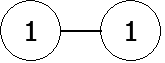
\includegraphics[height=30px]{ext/3.1.png}
                \caption{Здесь, \(x_i = 1, x_j = 1\), остальные 0.}
            \end{Graph}
            \begin{gather*}
            f(x) = 1^2 + 1^2 - (a_i + a_j) > 0 \Rightarrow 2 > (a_i + a_j). ?!?
            \end{gather*}
        \end{proof}
         Соответственно, строим граф на вершинах \((x_i)\) и двусторонних рёбрах.
    \subsection[\large{Рассмотрение компонент связности по отдельности}]{
    \large{Рассмотрение компонент связности по отдельности}\hypertarget{Component}{}
    }
        \begin{proof}{Каждую компоненту необходимо и достаточно рассматривать по отдельности} 
            Обозначим компоненту за C. \\
            Необходимость: $\letus$  $\forall \text{ } x_i \notin C , x_i = 0$.
            В таком случае, если для компоненты не выполняется то и для всего графа не выполняется. \\
            Обозначим количество компонент за c. \\
            Достаточность: Если выполняется для всех c компонент, то можем записать:
            \begin{gather*}
            \forall \text{ } i \leq c : f_i(x) > 0 \Rightarrow f(x) = \sum_{i=1}^c f_i(x) > 0
            \end{gather*}
        \end{proof}
        Также заметим, что в дальнейшем будут доказаны невыполнения условий для некоторых примеров, и этого будет достаточно, по причине того, что мы можем, аналогично этому доказательству, занулить вершины графа так, что останется подграф, необходимый нам, и случай невыполнения условия для него будет равносилен случаю невыполнения условия для всего графа. 
    \subsection{\large{Компонента является деревом}}
        \begin{proof}{Компонента графа является деревом} 
            Обозначим компоненту за C. \\
            Хотим доказать что C не содержит циклов.\\
            От противного:
            $
            \letus \text{ } \exists \text{ } (i_k) \subset C : \forall \text{ } 1 \leq r \leq k : (x_{i_r}, x_{i_{r+1}}) \in V \text{ и } (x_{i_k}, x_{i_1}) \in V.
            $\\
            Тогда, рассмотрим пример:
            \begin{Graph}
                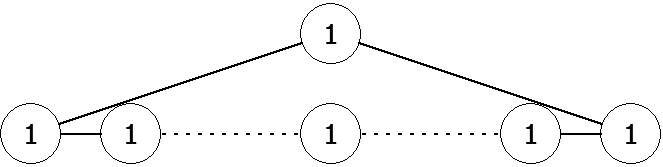
\includegraphics[height=60px]{ext/3.3.png} \\
                \caption{Здесь, $\forall \text{ } 1 \leq i \leq n : x_i = 1$}
            \end{Graph}
            Заметим, что тогда: \\
            \begin{gather*}
            f(x) = \sum_1^k 1^2 - \sum_1^k 1 * 1 = 0 \ngtr 0.?!?
            \end{gather*}
         \end{proof}
         
    \subsection{\large{Степень вершин \texorpdfstring{$\leq$ }{Lg} 3}}
        \begin{proof}{Нет вершин степени > 3}
            От противного:\\
            $\letus \text{ } \exists \text{ } i \leq n : deg(x_i) > 3.$ \\
            Тогда рассмотрим пример:
            \begin{Graph}
                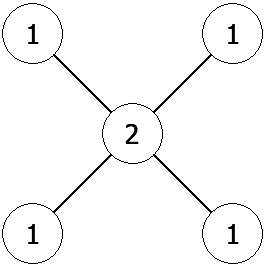
\includegraphics[height=90px]{ext/3.4.png} \\
                \caption{ Здесь, соседи вершины $x_i = 2: x_{j_1}, x_{j_2}, x_{j_3}, x_{j_4} = 1$ }
            \end{Graph}
            Тогда: \\ 
            \begin{gather*}    
            f(x)=\sum_1^41^2+2^2-\sum_1^42*1 = 8-8=0 \ngtr 0. ?!?
            \end{gather*}
        \end{proof}
    \subsection{\large{Вершин степени 3 не больше одной}}
        \begin{proof}{Вершин степени 3 $\leq$ 1}
            От противного:\\
            $\letus \text{ } \exists\text{ } i,j \leq n : deg(x_i) = 3 \text{ и } deg(x_j) = 3$ \\
            Также $\letus$ между ними ровно k вершин. \\
            Тогда рассмотрим пример:
            \begin{Graph}
                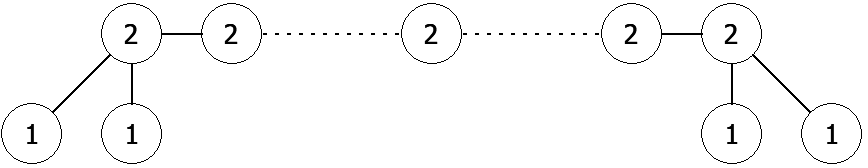
\includegraphics[height=60px]{ext/3.5.png} \\
                \caption{Где $x_i=x_j=2, \forall l \leq k : x_{r_l}=2, x_a=x_b=x_c=x_d=1$}
            \end{Graph}
            \begin{gather*}    
            f(x)=\sum_1^{k+2}2^2+\sum_1^41^2-\sum_1^41*2-\sum_1^{k+1}2*2=(k+2)*4+4-8-(k+1)*4\\=4+4-8=0 \ngtr 0. ?!?
            \end{gather*}
        \end{proof}
        Теперь можем представлять граф с помощью одной вершины степени три и трёх ``отростков``, из неё исходящих.
    \subsection{\large{Один из ``отростков`` графа имеет длину 1}}
        \begin{proof}{Один из ``отростков`` имеет длину $\leq$ 1}
            От противного: Предположим, что все ``отростки`` имеют длину хотя бы 2.\\
            Тогда рассмотрим пример:
            \begin{Graph}
                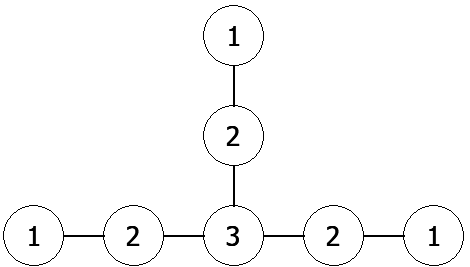
\includegraphics[height=90px]{ext/3.6.png} \\
                \caption{Здесь, $x_a=3, x_{b_1}=x_{b_2}=x_{b_3}=2, x_{c_1}=x_{c_2}=x_{c_3}=1$}
            \end{Graph}
            \begin{gather*}
            f(x)=3^2+3*2^2+3*1^2-3*2-3*6=9+12+3-6-18=0 \ngtr 0. ?!?
            \end{gather*}
        \end{proof}
    \subsection{\large{Один из оставшихся ``отростков`` имеет длину\texorpdfstring{ $\leq$ }{Lg} 3}}
        \begin{proof}{Хотя бы один из оставшихся ``отростков`` имеет длину $\leq$ 3}
            От противного: Предположим, что оба имеют длину $\geq$ 4.\\
            Тогда рассмотрим пример:
            \begin{Graph}
                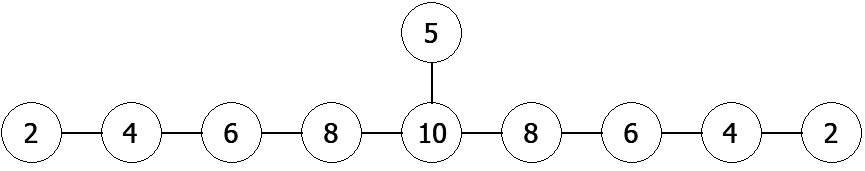
\includegraphics[height=70px]{ext/3.7.png} \\
                \caption{Здесь, $x_{i_1} = 10, x_{i_2}=x_{i_3}=8, x_{i_4}=x_{i_5}=6, x_{i_6} = x_{i_7}=4, x_{i_8}=x_{i_9}=2, x_{i_10}=5$}
            \end{Graph}
            \begin{gather*} 
            f(x)=2 * (2^2 + 4^2 + 6^2 + 8^2 + 10^2) + 5^5 - \\ 2 * (2 * 4 + 4 * 6 + 6 * 8 + 8 * 10) - 5 * 10 = -5 < 0. ?!?
            \end{gather*}
        \end{proof}
    \subsection{\large{Получение ответа}}
        Обозначим ответ на задачу, как тройку чисел \{a, b, c\}, каждое из которых обозначает длину ``отростка``, причём порядок не важен.\\
        Нахождение ответа делится на несколько пунктов:
        \begin{enumerate}
            \item Ответ вида \{1, 1, x\}, x - любое
            \item Ответ вида \{0, 0, x\}, x - любое
            \item Ответ вида \{1, 2, x\}, x $\leq$ 4
            \item Больше ответов не существует
        \end{enumerate}
        \subsubsection{Ответ вида \{1, 1, x\}}
            \begin{proof}{Граф с двумя ``отростками`` длины 1 является ответом}
                Рассмотрим рисунок:
                \begin{Graph}
                    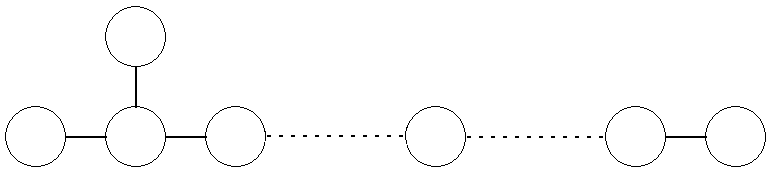
\includegraphics[height=60px]{ext/3.8.1.png}\\
                    \caption{Здесь, $(x_i), \text{ } y$.}
                \end{Graph}
                Запишем выражение:
                \begin{gather*}
                f(x)=\sum_{i=1}^n x_i^2 - \sum_{i=1}^{n-1} x_ix_{i+1} -x_2y = \\ 
                \sum_{i=n}^3 t_i(\frac{1}{2t_i}x_{i}-x_{i+1})^2+\frac{1}{4}(2y-x_2)^2 +\frac{1}{4}(2x_1-x_2)^2+C
                \end{gather*} Где C - какое-то значение (см. ниже), t - последовательность, определяющаяся как:
                \begin{gather*}
                t_{i+1}=\frac{1}{4(1-t_i)}, t_1=\frac{1}{4}
                \end{gather*}

                Чтобы доказать корректность равенства, сначала докажем Лемму.\\
                \begin{lemma}{\(t_i<\frac{1}{2}\)}
                    По индукции:\\
                    База: i = 1\\
                    \begin{gather*}
                    t_i = \frac{1}{4} < \frac{1}{2}
                    \end{gather*}
                    Переход: i $\rightarrow$ i+1 \\
                    $\letus\text{ } t_i=\frac{1}{2}-\frac{1}{a}, \text{ } a > 0$, тогда:
                    \begin{gather*}
                    t_{i+1}= \frac{1}{4(1-t_i)} = \frac{1}{4(\frac{1}{2}+\frac{1}{a})} = \frac{2a}{4(a+2)} = \frac{2a}{4a+8} = \frac{a}{2a+4}
                    \end{gather*} 
                    \begin{gather*} 
                    \Rightarrow t_{i+1}=\frac{1}{2}-\frac{1}{a+2}
                    \end{gather*}
                \end{lemma}
                
                Теперь рассмотрим пару соседних слагаемых:
                \begin{gather*}
                t_i ( \frac{1}{2t_i}x_i - x_{i+1})^2 + \frac{1}{4(1-t_i)} ( 2(1-t_i) x_{i+1} - x_{i+2})^2 = \\
                \frac{1}{4t_i^2}x_i^2 - x_ix_{i+1} + t_ix_{i+1}^2 + \frac{(1-t_i)^2}{(1-t_i)}x_{i+1}^2 - x_{i+1}x_{i+2} + \frac{1}{4(1-t_i)}x_{i+2}^2 = \\
                x_{i+1}^2 -x_ix_{i+1}-x_{i+1}x_{i+2} + \frac{1}{4t_i^2}x_i^2 + \frac{1}{4(1-t_i)}x_{i+2}^2
                \end{gather*}
                \hypertarget{fact1}{Заметим, что перед $x_{i+1}^2$, а также $-x_ix_{i+1}$ и $-x_{i+1}x_{i+2}$,  стоит коэффициент 1, а значит, что перед всеми квадратами и попарными произведениями будет стоять 1}, кроме слагаемого $x_2^2$. Для этого, определим C, как: 
                \begin{gather*}
                C =  (1-\frac{1}{4} -\frac{1}{4} - t_{n-2}^2)x_2^2 = (\frac{1}{2}-t_{n-2}^2)x_2^2.
                \end{gather*}
                Поскольку $t_{n-2} < \frac{1}{2}$ по лемме, то: 
                \begin{gather*}
                t_{n-2}^2 < \frac{1}{4} \Rightarrow C > 0 \rightarrow
                f(x) - \text{сумма квадратов} + C > 0 \Rightarrow f(x) > 0
                \end{gather*}
            \end{proof}
            То есть ответ \{1, 1, x\} - подходит.
        \subsubsection{Ответ вида \{0, 0, x\}}
            \begin{proof}{Бамбук любой длины является ответом}
                Запишем:
                \begin{gather*}f(x) = \frac{1}{2}x_1^2 + \sum_1^{n-1} \frac{1}{2}(x_i-x_{i+1})^2 + \frac{1}{2}x_n^2\end{gather*}
                $\Rightarrow f(x) > 0$, так как сумма квадратов и не все элементы нули.
            \end{proof}
        \subsubsection{Ответ вида \{1, 2, x\}, x \texorpdfstring{$\leq$ }{Lg} 4}
            \begin{proof}{Если один ``отросток`` имеет длину 2, то второй имеет длину $\leq 4$}
                От противного. \\
                Рассмотрим пример:
                \begin{Graph}
                    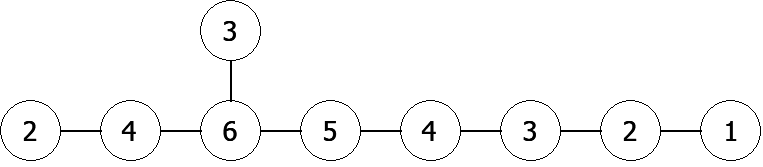
\includegraphics[height=60px]{ext/3.8.3.png}\\
                    \caption{Здесь, $x_{i_1}= x_{i_7}=2, x_{i_2}=x_{i_5}=4, x_{i_3}=6, x_{i_3}=6, x_{i_4}=5, x_{i_6}=y=3, x_{i_8}=1$.}
                \end{Graph}
                Тогда: 
                \begin{gather*} 
                f(x) = 2 * 2^2 + 2 * 4^2 + 6^2 + 2 * 3^2 + 5^2 + 1^2 -2 * 4 - 4 * 6 - \\ 6 *3 - 6 * 5 - 5 * 4 - 4 * 3 - 3 * 2 0 2 * 1 = 120 - 120 = 0 \ngtr 0. ?!?
                \end{gather*}
            \end{proof}
            \begin{proof}{Достаточность предыдущего утверждения}
                \begin{gather*} 
                f(x) = \sum_n^{4}t_i(\frac{1}{2t_i}x_i-x_{i+1})^2 + \frac{1}{4}(2y-x_3)^2+\sum_1^2t_i(\frac{1}{2t_i}x_i-x_{i+1})^2 + C
                \end{gather*} Где C - какая-то величина.\\
                Тогда выполняются \hyperlink{fact1}{все те же утверждения}, кроме коэффициента перед $x_3^2$:
                $t_2+t_{n-3}+\frac{1}{4}$.
                Выпишем первые четыре $t_i$:
                \(t_1 = \frac{1}{4}, t_2=\frac{1}{3}, t_3=\frac{3}{8}, t_4=\frac{2}{5}\).\\
                Заметим, что так как длина ``отростка`` $\leq 4$, то $t_{n-3} \leq t_4 \Rightarrow$ максимальная сумма:\\
                \(t_2+t_4+\frac{1}{4} = \frac{1}{3} + \frac{2}{5} + \frac{1}{4} =\frac{59}{60} \Rightarrow\) коэффициент перед $x_3^2 < 1 \Rightarrow C > 0 \Rightarrow$ $f(x) > 0$.
            \end{proof}
        \subsubsection{Больше ответов не существует}
            \begin{proof}{Если ``отросток`` имеет длину хотя бы 3, то второй будет иметь длину $\leq$ 2}
                Рассмотрим пример:
                \begin{Graph}
                    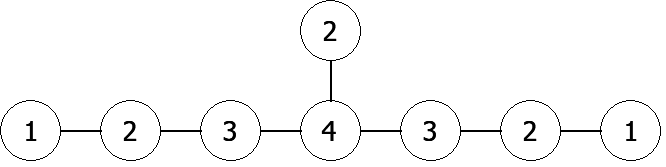
\includegraphics[height=60px]{ext/3.8.4.png}\\
                    \caption{ Здесь, $x_{i_1}=x_{i_7}=1, x_{i_2}=x_{i_6}=2, x_{i_3}=x_{i_5}=3, x_{i_4}=4, y=2$.}
                \end{Graph}
                \(f(x)=2*1^2+3*2^2+2*3^3+4^2 - 2 * (1 * 2 + 2 * 3 + 3 * 4) - 2 * 4 = 48 - 48 = 0 \ngtr 0\) ?!?
            \end{proof}
            Заметим, что тогда такие ответы, с точностью до отражения, мы уже рассматривали в пунктах 3.8.1 и 3.8.3
        \subsubsection{Итоговый ответ.}
            Подходят графы, состоящие из компонент связности вида \{0, 0, x\}, x - любое; \{1, 1, x\}, x - любое; \{1, 2, x\}, $x \leq 4$.
    \pagebreak
    
    \section{\textsc{Классификация неотрицательных форм}}
        Шаги решения:
        \begin{enumerate}
            \item $a_{ij} + a_{ji} \leq 2$, причем при равенстве всего 1 ответ. Можем рассматривать как граф.
            \item Рассматриваем компоненты связности по отдельности.
            \item Каждая компонента дерево либо цикл.
            \item Все вершины имеют степень $\leq 4$.
            \item Вершин степени 4 не больше одной.
            \item Если есть все 4 ``отростка``, то их длины ровно 1.
            \item Итоговый ответ.
        \end{enumerate}
        
        \subsection{\large{Можем рассматривать как граф}}
            \subsubsection{\texorpdfstring{$a_{ij} + a_{ji} \leq 2$}{Lg}}
                \begin{proof}{\texorpdfstring{$a_{ij} + a_{ji} \leq 2$}{Lg}}
                    Рассмотрим пример:
                    \begin{Graph}
                        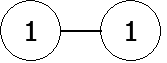
\includegraphics[height=30px]{ext/4.1.1.png}\\
                        \caption{ Здесь, $x_i=x_j=1$}
                    \end{Graph}
                    Тогда: 
                    \begin{gather*}
                    f(x)=1^2+1^2-(a_{ij}+a_{ji})<0. ?!?
                    \end{gather*}
                \end{proof}
            \subsubsection{При равенстве всего 1 пример}
                \begin{proof}{При равенстве всего 1 пример}
                    Предположим, что в такой компоненте хотя бы 3 вершины.
                    Тогда рассмотрим пример:
                    \begin{Graph}
                        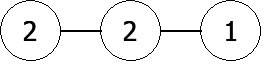
\includegraphics[height=30px]{ext/4.1.2.png}\\
                        \caption{ Здесь, $x_{i_1}=x_{i_2}=2, x_{i_3}=1$.}
                    \end{Graph}
                    Тогда: 
                    \begin{gather*}
                    f(x)=2*2^2+1^2-2*2*2-2*1*(a_{ij}+a_{ji})=1-2*(a_{ij}+a_{ji}) < 0. ?!?
                    \end{gather*}
                \end{proof}
        \subsection{\large{Рассмотрение компонент связности по отдельности.}}
            Аналогично пункту \hyperlink{Component}{3.2}
        \subsection{\large{Каждая компонента -- дерево либо цикл.}}
            \begin{proof}{Каждая компонента -- дерево либо цикл.}
                От противного.\\
                Пусть в компоненте есть цикл и ещё 1 вершина или ребро вне него.\\
                Если вершина, тогда рассмотрим пример:
                \begin{Graph}
                    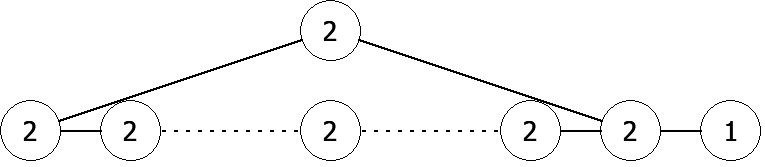
\includegraphics[height=60px]{ext/4.2.png}\\
                    \caption{Здесь, $\forall i \leq n : x_i=2, y=1$}
                \end{Graph}
                Тогда: 
                \begin{gather*}
                f(x)=k*2^2+1^2-2*2*k-2*1=-1 < 0. ?!?
                \end{gather*}
                Если ребро, тогда, взяв все вершины за 1:
                \begin{gather*}
                f(x)=k*1^2-k*1^2-1*1*1=-1 < 0. ?!?
                \end{gather*}
            \end{proof}
        \subsection{\large{Все вершины имеют степень \texorpdfstring{$\leq$ }{Lg} 4}}
            {\begin{proof}{Все вершины имеют степень \texorpdfstring{$\leq$ }{Lg} 4}
                От противного.\\
                Тогда рассмотрим пример:
                \begin{Graph}
                    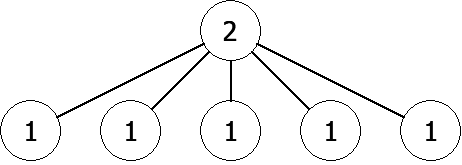
\includegraphics[height=60px]{ext/4.3.png}\\
                    \caption{Здесь, $x_1=x_2=x_3=x_4=x_5=1, y=2$.}
                \end{Graph}
                Тогда: 
                \begin{gather*}
                f(x)=5*1^2+2^2-2*1*5=9-10=-1<0. ?!?
                \end{gather*}
            \end{proof}
        \subsection{\large{Вершин степени 4 не больше одной.}}
            \begin{proof}{Вершин степени 4 не больше одной.}
                От противного.\\
                Рассмотрим пример:
                \begin{Graph}
                    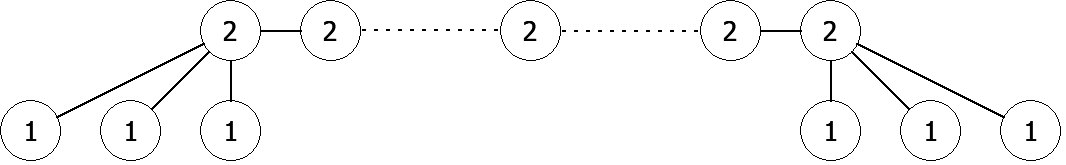
\includegraphics[height=60px]{ext/4.5.png}\\
                    \caption{Здесь,  $y_1=y_2= ... = y_6=1, x_1=x_2 = ... = x_k=2$}
                \end{Graph}
                Тогда: 
                \begin{gather*}
                f(x)=6*1^2+k*2^2-(k-1)*2*2-2*6=-2<0. ?!?
                \end{gather*}
            \end{proof}
        \subsection{\large{Если есть все 4 ``отростка``, то их длины ровно 1.}}
            \begin{proof}{Если есть все 4 ``отростка``, то их длины ровно 1.}
                От противного.\\
                Рассмотрим пример:
                \begin{Graph}
                    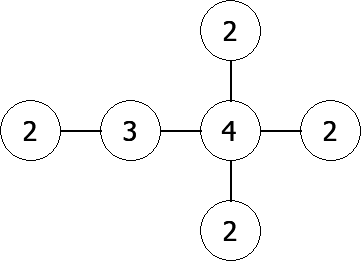
\includegraphics[height=90px]{ext/4.6.png}\\
                    \caption{Здесь, $x_{i_1}=4, x_{i_2}=3, x_{i_3}=x_{i_4}=x_{i_5}=2$}
                \end{Graph}
                Тогда: 
                \begin{gather*}
                f(x)=4*2^2+3^3+4^2-2*3-3*4-4*2*3=-1<0. ?!?
                \end{gather*}
            \end{proof}
        \subsection{\large{Итоговый ответ.}}
            Ответами будут являться компоненты связности вида: цикла; двух вершин с ребром 2; вершины с четырьмя детьми; того же набора компонент, что и для положительных форм.
    \pagebreak

    \section{\textsc{Графы решений положительных форм}}
        Будем рассматривать графы решений уравнения $f(x) = 1$.\\
        Шаги решения:\\
        \begin{enumerate}
            \item Решения форм вида \{0, 0, x\}
            \item Графы решений форм вида \{0, 0, x\}
            \item Решения форм вида \{1, 1, x\}
            \item Графы решений форм вида \{1, 1, x\}
            \item Решения форм вида \{1, 2, x\}
            \item Графы решений форм вида \{1, 2, x\}
            \item Следствия
        \end{enumerate}
        
        \subsection{\large{Решения форм вида \{0, 0, x\}}}
            Рассмотрим запись такой формы:
            \begin{gather*}
            f(x)=\sum_1^n x_i^2 - \sum_1^{n-1} x_ix_{i+1} = \sum_1^{n-1} \frac{1}{2}(x_i-x_{i+1})^2 +\frac{1}{2}x_1^2 + \frac{1}{2}x_n^2 = 1
            \end{gather*}
            \begin{gather*}
            \sum_1^{n-1} (x_i-x_{i+1})^2 + x_1^2 + x_n^2 = 2
            \end{gather*}
            Обозначим пару $(x_i, x_{i+1})$ переходом, если $|x_i-x_{i+1}| = 1$.\\
            Также стоит заметить, что $\nexists \text{ } i : |x_i-x_{i+1}| > 1$, так как, тогда вся сумма выражения будет $\geq$ 4. По аналогичным соображениям $|x_1|$ < 2 и $|x_n|$ < 2. Тогда, поскольку все числа целые и квадраты неотрицательны, то достаточно рассмотреть лишь несколько случаев:
            \begin{enumerate}
                \item $x_1 = \pm 1, x_n=\pm 1$, переходов 0.
                \item $x_1 = \pm1, x_n=0$, переход 1.
                \item $x_1 = 0, x_n=\pm 1$, переход 1.
                \item $x_1 = 0, x_n = 0$, переходов 2.
            \end{enumerate}
            \subsubsection{\texorpdfstring{$x_1 = \pm 1, x_n=\pm 1$}{Lg}, переходов 0.}
                Заметим, что поскольку переходов 0, то все числа равны. Откуда следует, что $x_1 = x_n$.\\
                Поэтому получаем два ответа: $\forall \text{ } 1 \leq i \leq n : x_i=1$ и $\forall \text{ } 1 \leq i \leq n : x_i=-1$.
            \subsubsection{\texorpdfstring{$x_1 = \pm1, x_n = 0$}{Lg}, переход 1.}
                Поскольку переход всего 1, то получаем возможные ответы, как массив из 1 или -1, конкатенированный с массивом из 0.
                То есть ответы вида: $\exists \text{ } 1 \leq i < n : \forall \text{ } 1 \leq j \leq i : x_j=1, \forall \text{ } i < j \leq n : x_j=0$ и $\exists \text{ } 1 \leq i < n : \forall \text{ } 1 \leq j \leq i : x_j=-1, \forall \text{ } i < j \leq n : x_j=0$
            \subsubsection{\texorpdfstring{$x_1 = 0, x_n=\pm 1$, переход 1.}{Lg}}
                Аналогично предыдущему пункту получаем ответы: $\exists \text{ } 1 < i \leq n : \forall \text{ } 1 \leq j < i : x_j=0, \forall \text{ } i \leq j \leq n : x_j=1$ и $\exists \text{ } 1 < i \leq n : \forall \text{ } 1 \leq j < i : x_j=0, \forall \text{ } i \leq j \leq n : x_j=-1$
            \subsubsection{\texorpdfstring{$x_1 = 0, x_n = 0$}{Lg}, переходов 2.}
                Заметим, что данный набор аналогичен тому, что $\exists \text{ } 1 < i \leq j < n : \forall \text{ } i \leq k \leq j : x_k = 1$ или $\exists \text{ } 1 < i \leq j < n : \forall \text{ } i \leq k \leq j : x_k = -1$.\\
            \\
            Из всех данных случаев получаем, что единственным и достаточным условием ответа является массив из нулей, содержащий в себе подмассив из 1 или -1. То есть общее решение выглядит, как:
            \begin{gather*}\exists \text{ } 1 \leq i \leq j \leq n : \forall \text{ } i \leq k \leq j : x_k = 1 \lor \exists \text{ } 1 \leq i \leq j \leq n : \forall \text{ } i \leq k \leq j : x_k = -1.\end{gather*}
        \subsection{\large{Графы решений форм вида \{0, 0, x\}}}
            Зная множество решений этой формы, можно заметить что граф слабоположительных решений, будет выглядеть, как граф, у каждой вершины которого 2 родителя и 2 ребёнка, за исключением, вершины корня (решения из всех 1), и вершин листьев, решения с одной 1).
            \begin{Graph}
                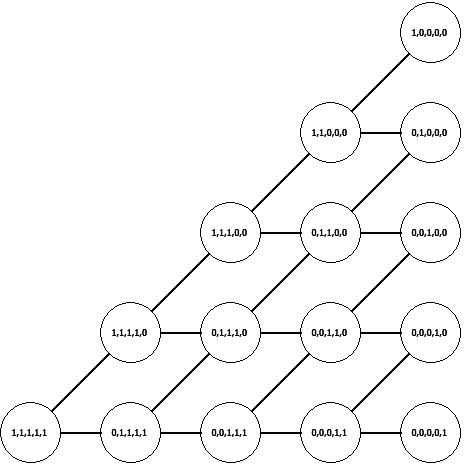
\includegraphics[height=230px]{ext/5.2.1.png}\\
                \caption{Граф слабоположительных решений для x = 5.}
                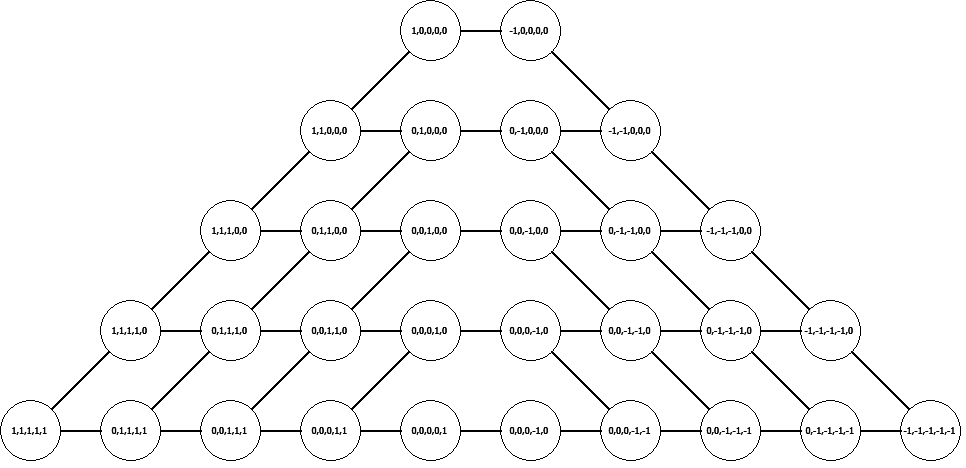
\includegraphics[height=230px]{ext/5.2.2.png}\\
                \caption{Граф всех решений для x = 5.}
            \end{Graph}
        \subsection{\large{Решения форм вида \{1, 1, x\}}}
             Рассмотрим запись такой формы:
            \begin{gather*}
            f(x)=\sum_1^n x_i^2 - \sum_1^{n-1} x_ix_{i+1} - x_2y = \sum_2^{n-1} \frac{1}{4}(x_i-x_{i+1})^2 +\frac{1}{4}(2x_1-x_2)^2 + \frac{1}{4}(2y-x_2)^2 + \frac{1}{2} x_n^2 = 1
            \end{gather*}
            \begin{gather*}
            \sum_2^{n-1} 2(x_i-x_{i+1})^2 + 2x_n^2 + (2x_1-x_2)^2+(2y-x_2)^2 = 4
            \end{gather*}
            Обозначим пару $(x_i, x_{i+1})$ переходом, если $|x_i-x_{i+1}| = 1$.\\
            Тогда, достаточно рассмотреть несколько случаев:\\
            \begin{enumerate}
                \item $x_n^2 = 0$
                \begin{enumerate}
                    \item 
                    $
                        \begin{cases}
                            (2x_1-x_2)^2=1\\
                            (2y-x_2^2)^2=1\\
                            1 \text { переход}
                        \end{cases}
                    $
                    \item 
                    $
                        \begin{cases}
                            (2x_1-x_2)^2=4\\
                            (2y-x_2^2)^2=0\\
                            0 \text { переходов}
                        \end{cases}
                    $
                    \item 
                    $
                        \begin{cases}
                            (2x_1-x_2)^2=0\\
                            (2y-x_2^2)^2=4\\
                            0 \text { переходов}
                        \end{cases}
                    $
                    \item 
                    $
                        \begin{cases}
                            (2x_1-x_2)^2=0\\
                            (2y-x_2^2)^2=0\\
                            2 \text { перехода}
                        \end{cases}
                    $
                \end{enumerate}
                \item $x_n=1$
                \begin{enumerate}
                    \item 
                    $
                        \begin{cases}
                            (2x_1-x_2)^2=1\\
                            (2y-x_2)^2=1\\
                            0 \text{ переходов}
                        \end{cases}
                    $
                    \item 
                    $
                        \begin{cases}
                            (2x_1-x_2)^2=0\\
                            (2y-x_2^2)^2=0\\
                            1 \text{ переход}
                        \end{cases}
                    $
                \end{enumerate}
                \item $x_n=-1$
                \begin{enumerate}
                    \item 
                    $
                        \begin{cases}
                            (2x_1-x_2)^2=1\\
                            (2y-x_2)^2=1\\
                            0 \text{ переходов}
                        \end{cases}
                    $
                    \item 
                    $
                        \begin{cases}
                            (2x_1-x_2)^2=0\\
                            (2y-x_2^2)^2=0\\
                            1 \text{ переход}
                        \end{cases}
                    $
                \end{enumerate}
            \end{enumerate}
        \subsubsection{}
            $
                \begin{cases}
                    x_n=0\\
                    (2x_1-x_2)^2=1\\
                    (2y-x_2^2)^2=1\\
                    1 \text{ переход}
                \end{cases}
            $\\
            Поскольку $x_n=0$, то есть два варианта: переход вида (1, 0) и (-1, 0), поэтому $x_2=\pm1$. Откуда $2x_1=\pm1\pm1 \Rightarrow x_1=0 \text{ или } x_1=x_2$. Аналогично $2y=\pm1\pm1 \Rightarrow y=0 \text{ или } y=x_2$. Соответственно решения будут выглядеть, как массив нулей с подмассивом 1 или -1 и отдельно заданными $x_1$ и $y$, то есть: 
            \begin{gather*}
            \exists \text{ } 2 \leq i \leq n-1 : \forall \text{ } 2 \leq k \leq i : x_k = 1, \text{ } x_1 = \begin{sqcases} 0 \\ 1 \end{sqcases}, \text{ } y = \begin{sqcases} 0 \\ 1 \end{sqcases}\\
             \exists \text{ } 2 \leq i \leq n-1 : \forall \text{ } 2 \leq k \leq i : x_k = -1, \text{ } x_1 = \begin{sqcases} 0 \\ -1 \end{sqcases}, \text{ } y = \begin{sqcases} 0 \\ -1 \end{sqcases}
             \end{gather*}
        \subsubsection{}
            $
            \begin{cases}
                x_n = 0\\
                (2x_1-x_2)^2=4\\
                (2y-x_2^2)^2=0\\
                0 \text { переходов}
            \end{cases}
            $\\
            Заметим, что так как переходов 0, то $x_2=x_n=0 \Rightarrow x_1 = 0, \text{ } 2y=\pm2 +x_2 \Rightarrow y=x_2\pm1=\pm1.$ Тогда ответом является:
            \begin{gather*}
            \forall \text{ } 1 \leq i \leq n : x_i=0, \text{ } y = 1.
            \\
            \forall \text{ } 1 \leq i \leq n : x_i=0, \text{ } y = -1.
            \end{gather*}
        \subsubsection{} 
            $
            \begin{cases}
                x_n=0\\
                (2x_1-x_2)^2=0\\
                (2y-x_2^2)^2=4\\
                0 \text { переходов}
            \end{cases}
            $\\
            Аналогично предыдущему пункту получаем ответы:
            \begin{gather*}
            \forall \text{ } 2 \leq i \leq n : x_i=0, \text{ } y = 0, \text{ } x_1 = 1
            \\
            \forall \text{ } 2 \leq i \leq n : x_i=0, \text{ } y = 0, \text{ } x_1 = -1
            \end{gather*}
        \subsubsection{}
            $
                \begin{cases}
                    x_n = 0\\
                    (2x_1-x_2)^2=0\\
                    (2y-x_2^2)^2=0\\
                    2 \text { перехода}
                \end{cases}
            $\\
            Из второго и третьего равенства получаем, что $x_1=y=\frac{x_2}{2}$.
            Также поскольку переходов ровно 2, то всего четыре случая: когда есть переходы (1, 0) и (2, 1); (1, 0) и (0, 1); (-1, 0) и (-2, -1); (-1, 0) и (0, -1). То есть существуют решения вида:\\
            $
            \exists \text{ } 2 \leq i \leq n-1 : \forall \text{ } 2 \leq k \leq i : x_k=2, \text{ } \forall \text{ } i < k \leq j : x_k = 1, \\ \forall \text{ } j < k \leq n : x_k=0, \text{ } x_1=y=1 
            $ \\ и \\
            $
            \exists \text{ } 2 \leq i < j \leq n-1 : \forall \text{ } 2 \leq k \leq i : x_k=0, \text{ } \forall \text{ } i < k \leq j : x_k = 1, \\ \forall \text{ } j < k \leq n : x_k=0, \text{ } x_1=y=0
            $\\ и \\
            $
            \exists \text{ } 2 \leq i < j \leq n-1 : \forall \text{ } 2 \leq k \leq i : x_k=-2, \text{ } \forall \text{ } i < k \leq j : x_k = -1, \\ \forall \text{ } j < k \leq n : x_k=0, \text{ } x_1=y=-1 
            $\\ и \\
            $
            \exists \text{ } 2 \leq i < j \leq n-1 : \forall \text{ } 2 \leq k \leq i : x_k=0, \text{ } \forall \text{ } i < k \leq j : x_k = -1, \\ \forall \text{ } j < k \leq n : x_k=0, \text{ } x_1=y=0 
            $
        \subsubsection{}
            $
                \begin{cases}
                    x_n=1\\
                    (2x_1-x_2)^2=1\\
                    (2y-x_2)^2=1\\
                    0 \text{ переходов}
                \end{cases}
            $\\
            Так как переходов 0, то $x_2 = 1$, а также $2x_1=1\pm1$ и $2y=1\pm1 \Rightarrow x_1=\begin{sqcases}0\\1\\\end{sqcases}$ и $y= \begin{sqcases}0\\1\\\end{sqcases}$. То есть решениями являются:\\
            $
            \forall \text{ } 2 \leq i \leq n : x_i=1, \text{ } x_1 = 0, \text{ } y = 0.
            $\\ и \\
            $
            \forall \text{ } 2 \leq i \leq n : x_i=1, \text{ } x_1 = 1, \text{ } y = 0.
            $\\ и \\
            $
            \forall \text{ } 2 \leq i \leq n : x_i=1, \text{ } x_1 = 0, \text{ } y = 1.
            $\\ и \\
            $
            \forall \text{ } 2 \leq i \leq n : x_i=1, \text{ } x_1 = 1, \text{ } y = 1.
            $
        \subsubsection{}
            $
                \begin{cases}
                    x_n=1\\
                    (2x_1-x_2)^2=0\\
                    (2y-x_2^2)^2=0\\
                    1 \text{ переход}
                \end{cases}
            $\\
            Так как переход 1, то есть два варианта: $x_2 = 0$ и $x_2=2$.
            В первом случае $x_1 = y = 0$, во втором $x_1=y=1$. То есть решениями являются:
            $
            \exists \text{ } 2\leq i \leq n-1 : \forall \text{ } 1 \leq k < i : x_k=0, \forall \text{} i \leq k \leq n : x_k = 1, \text{ } y = 0. 
            $\\ и \\
            $
            \exists \text{ } 2\leq i \leq n-1 : \forall \text{ } 2 \leq k < i : x_k=2, \forall \text{ } i \leq k \leq n : x_k = 1, \text{ } y = x_1 = 1. 
            $
        \subsubsection{}
            $
                \begin{cases}
                    x_n=-1\\
                    (2x_1-x_2)^2=1\\
                    (2y-x_2)^2=1\\
                    0 \text{ переходов}
                \end{cases}
            $\\
            Аналогично, решения:\\
            $
            \forall \text{ } 2 \leq i \leq n : x_i=-1, \text{ } x_1 = 0, \text{ } y = 0.
            $\\ и \\
            $
            \forall \text{ } 2 \leq i \leq n : x_i=-1, \text{ } x_1 = -1, \text{ } y = 0.
            $\\ и \\
            $
            \forall \text{ } 2 \leq i \leq n : x_i=-1, \text{ } x_1 = 0, \text{ } y = -1.
            $\\ и \\
            $
            \forall \text{ } 2 \leq i \leq n : x_i=-1, \text{ } x_1 = -1, \text{ } y = -1.
            $
        \subsubsection{}
            $
                \begin{cases}
                    x_n=-1\\
                    (2x_1-x_2)^2=0\\
                    (2y-x_2^2)^2=0\\
                    1 \text{ переход}
                \end{cases}
            $\\
            Аналогично, решения:\\
            $
            \exists \text{ } 2\leq i \leq n-1 : \forall \text{ } 1 \leq k < i : x_k=0, \forall \text{ } i \leq k \leq n : x_k = -1, \text{ } y = 0. 
            $\\ и \\
            $
            \exists \text{ } 2\leq i \leq n-1 : \forall \text{ } 2 \leq k < i : x_k=-2, \forall \text{ } i \leq k \leq n : x_k = -1, \text{ } y = x_1 = -1. 
            $

        
        \subsection{\large{Графы решений форм вида \{1, 1, x\}}}
            Граф решений такой формы, очевидно, будет содержать в себе граф решений бамбуковой формы(который частично образуют все рассмотренные случаи 5.3), а также будут существовать решения, содержащие в себе префикс из 1 или -1 и $y = \begin{sqcases}1\\-1\end{sqcases}$ соответственно.
            Кроме того, будет ещё 1 тип решений: конкатенация массивов [1], массива из 2, массива из 1, массива из 0, и $y = 1$. И соответствующий ему массив с отрицательными значениями. \\
            Тогда граф решений можно представить как расширение графа решений бамбуковой формы, в котором будет надстроен граф над вершиной корнем, в котором рёбра ведущие снизу вверх заменяют 1 на 0, а слева направо заменяют 1 на 2.
            \begin{Graph}
                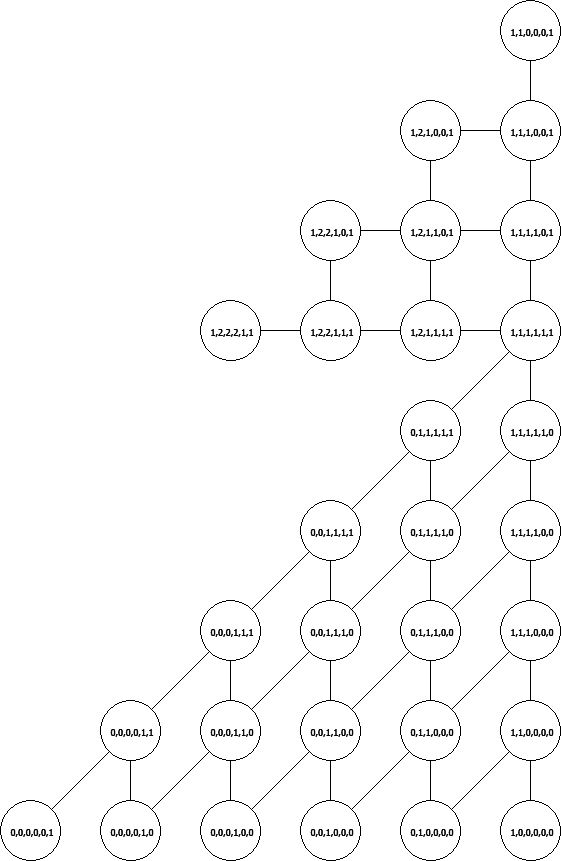
\includegraphics[height=500px]{ext/5.4.1.png}\\
                \caption{Граф слабоположительных решений для формы \{1, 1, 3\}}
            \end{Graph}
            \begin{Graph}
                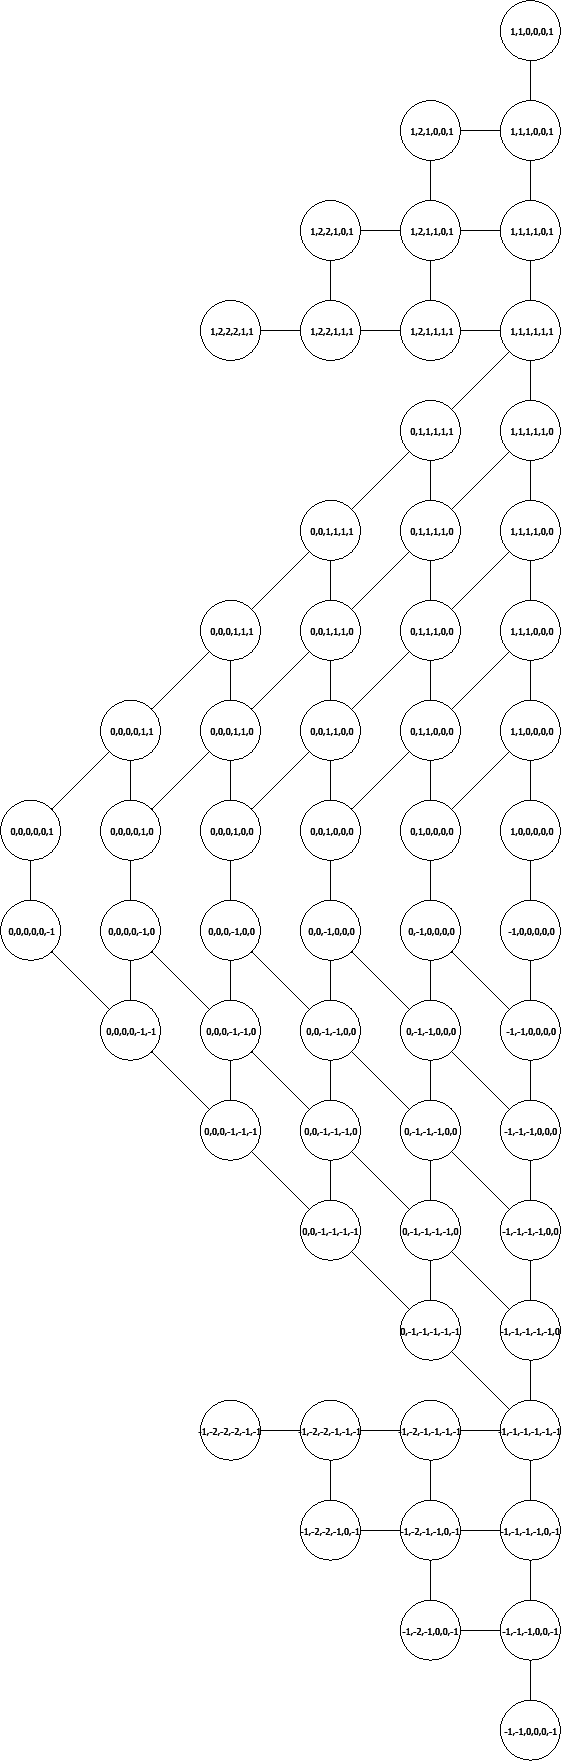
\includegraphics[height=500px]{ext/5.4.2.png}\\
                \caption{Граф всех решений для формы \{1, 1, 3\}}
            \end{Graph}
    \subsection{\large{Решения форм вида \{1, 2, x\}}}
        Мы будем рассматривать:
        \begin{enumerate} 
            \item Граф решений и решения формы \{1, 2, 2\} 
            \item Граф решений и решения формы \{1, 2, 3\} 
            \item Граф решений и решения формы \{1, 2, 4\}
        \end{enumerate}
        Представления решений этих форм возможно только с перебором большого количества вариантов, приводить который не является необходимым. Поэтому было доказано, что значения вершин в решениях лежат в определенном диапазоне, и был проведён компьютерный перебор, для нахождения решений и рёбер между ними.
    \subsection{\large{Граф решений и решения формы \{1, 2, 2\}}}
        \begin{proof}{В решении этой формы все числа лежат в отрезке [-3, 3]}
            Запишем сумму квадратов для этой формы:
            \begin{gather*}
                f(x)=x_1^2+x_2^2+x_3^2+x_4^2+x_5^2+y^2 \\
                -x_1x_2-x_2x_3-x_3x_4-x_4x_5-x_3y = 1 
            \end{gather*} 
            \begin{gather*}
                f(x) = \frac{1}{4} (2y-x_3)^2+\frac{1}{4} (2x_5-x_4)^2 + \frac{1}{3} (\frac{3}{2} x_4 - x_3)^2 +\\ \frac{1}{4} (2x_1-x_2)^2 + \frac{1}{3} (\frac{3}{2} x_2 - x_3)^2 + \frac{1}{12} x_3^2 = 1
            \end{gather*}
            \begin{gather*}
                3(2y-x_3)^2+3(2x_5-x_4)^2 + (3x_4 - 2x_3)^2 + 3(2x_1-x_2)^2 + (3 x_2 - 2x_3)^2 + x_3^2 = 12
            \end{gather*}
            Из этой суммы, следует что: \\
            $|x_3| \leq 3 \Rightarrow 
            \begin{cases}
                3x_2 \leq 3 + 2x_3 \leq 9 \rightarrow x_2 \leq 3 \\
                3x_2 \geq -3 + 2x_3 \geq -9 \rightarrow  x_2 \geq -3 \\
                3x_4 \leq 3 + 2x_3 \leq 9 \rightarrow x_4 \leq 3 \\
                3x_4 \geq -3 + 2x_3 \geq -9 \rightarrow  x_4 \geq -3 \\
                2y \leq 2 + x_3 \leq 5 \rightarrow y \leq 2 \\
                2y \geq 2 + x_3 \geq -5 \rightarrow y \geq -2
            \end{cases} \Rightarrow
            \begin{cases}
                2x_1 \leq 2 + x_2 \leq 5 \rightarrow x_1 \leq 2 \\
                2x_1 \geq -2 + x_2 \geq -5 \rightarrow x_1 \geq -2 \\
                2x_5 \leq 2 + x_4 \leq 5 \rightarrow x_5 \leq 2 \\
                2x_5 \geq -2 + x_4 \geq -5 \rightarrow x_5 \geq -2 \\
            \end{cases}
            $
        \end{proof}
         Решения: Смотри \hyperlink{table1}{таблицу 1} .

    \subsection{\large{Граф решений и решения формы \{1, 2, 3\}}}
        \begin{proof}{В решении этой формы все числа лежат в отрезке [-4, 4]}
            Запишем сумму квадратов для этой формы:
            \begin{gather*}
                f(x)=x_1^2+x_2^2+x_3^2+x_4^2+x_5^2+x_6^2+y^2 \\
                - x_1x_2-x_2x_3-x_3x_4-x_4x_5-x_5x_6-x_3y = 1 
            \end{gather*} 
            \begin{gather*}
                f(x) = \frac{1}{4} (2y-x_3)^2+\frac{1}{4} (2x_6-x_5)^2 + \frac{1}{3} (\frac{3}{2} x_5 - x_4)^2 + \\
                \frac{3}{8} (\frac{4}{3} x_4 - x_3)^2 +  \frac{1}{4} (2x_1-x_2)^2 +  \frac{1}{3} (\frac{3}{2} x_2 - x_3)^2 + \frac{1}{24} x_3^2 = 1
            \end{gather*}
            \begin{gather*}
                6(2y-x_3)^2+6(2x_6-x_5)^2 +2(3x_5 - 2x_4)^2 + \\ (4x_4 - 3x_3)^2 +  6(2x_1-x_2)^2 + 2(3x_2 - 2x_3)^2 + x_3^2 = 24
            \end{gather*}
            Из этой суммы, следует что: 
            \begin{gather*}|x_3| \leq 4 \Rightarrow\end{gather*}
            \begin{gather*} 
            \begin{cases}
                3x_2 \leq 3 + 2x_3 \leq 11 \rightarrow x_2 \leq 3 \\
                3x_2 \geq -3 + 2x_3 \geq -11 \rightarrow  x_2 \geq -3 \\
                4x_4 \leq 3 + 3x_3 \leq 15 \rightarrow x_4 \leq 3 \\
                4x_4 \geq -3 + 3x_3 \geq -15 \rightarrow  x_4 \geq -3 \\
                2y \leq 2 + x_3 \leq 6 \rightarrow y \leq 3 \\
                2y \geq 2 + x_3 \geq -6 \rightarrow y \geq -3
            \end{cases} \Rightarrow \end{gather*}
            \begin{gather*}
            \begin{cases}
                2x_1 \leq 2 + x_2 \leq 5 \rightarrow x_1 \leq 2 \\
                2x_1 \geq -2 + x_2 \geq -5 \rightarrow x_1 \geq -2 \\
                3x_5 \leq 3 + 2x_4 \leq 9 \rightarrow x_5 \leq 3 \\
                3x_5 \geq -3 + 2x_4 \geq -9 \rightarrow x_5 \geq -3 \\
            \end{cases} \Rightarrow \end{gather*}
            \begin{gather*}
            \begin{cases}
                2x_6 \leq 2 + x_5 \leq 5 \rightarrow x_6 \leq 2 \\ 
                2x_6 \geq -2 + x_5 \leq -5 \rightarrow x_6 \geq -2 \\ 
            \end{cases}
            \end{gather*}
        \end{proof}
         Решения: Смотри \hyperlink{table2}{таблицу 2}.
    
    \subsection{\large{Граф решений и решения формы \{1, 2, 4\}}}
        \begin{proof}{В решении этой формы все числа лежат в отрезке [-7, 7]}
            Запишем сумму квадратов для этой формы:
           \begin{gather*}
            f(x)=x_1^2+x_2^2+x_3^2+x_4^2+x_5^2+x_6^2+x_7^2+y^2 -\\ x_1x_2-x_2x_3-x_3x_4-x_4x_5-x_5x_6-x_3y = 1 
            \end{gather*} 
            \begin{gather*}
            f(x) = \frac{1}{4} (2x_1-x_2)^2+\frac{1}{3} (\frac{3}{2}x_2-x_3)^2 + \frac{1}{4} (2y - x_3)^2 + \frac{1}{4} (2x_7 - x_6)^2 + \\  \frac{1}{3} (\frac{3}{2}x_6-x_)5^2 + \frac{3}{8} (\frac{4}{3} x_5 - x_4)^2
            + \frac{2}{5} (\frac{5}{3}x_4-x_3)^2 + \frac{1}{60} x_3^2 = 1
            \end{gather*}
            \begin{gather*}
            30(2x_1-x_2)^2+40(\frac{3}{2}x_2-x_3)^2 + 30(2y - x_3)^2 + 30(2x_7 - x_6)^2 + \\ 40(\frac{3}{2}x_6-x_)5^2 + 45(\frac{4}{3} x_5 - x_4)^2 + 48(\frac{5}{4}x_4-x_3)^2 + 2x_3^2 = 120
            \end{gather*}
            \begin{gather*}
            30(2x_1-x_2)^2+10(3x_2-2x_3)^2 + 30(2y - x_3)^2 + 30(2x_7 - x_6)^2 +\\ 10(3x_6-2x_5)^2 + 5(4x_5 - 3x_4)^2 + 3(5x_4-4x_3)^2 + 2x_3^2 = 120
            \end{gather*}
            Из этой суммы, следует что: 
            \begin{gather*}|x_3| \leq 7 \Rightarrow\end{gather*}
            \begin{gather*} 
            \begin{cases}
                (3x_2-2x_3)^2 \leq 12 \rightarrow 
                \begin{cases} 
                3x_2\leq 3 + 2x_3 \leq 17 \rightarrow x_2 \leq 5 \\
                3x_2 \geq -3 + 2x_3 \geq -17 \rightarrow  x_2 \geq -5
                \end{cases}\\
                (5x_4-4x_3)^2 \leq 40 \rightarrow 
                \begin{cases} 
                5x_4 \leq 6 + 4x_3 \leq 34 \rightarrow x_4 \leq 6 \\
                5x_4 \geq -6 + 4x_3 \geq -34 \rightarrow  x_4 \geq -6
                \end{cases}\\
                (2y-x_3)^2 \leq 4 \rightarrow
                \begin{cases}
                2y \leq 2 + x_3 \leq 9 \rightarrow y \leq 4 \\
                2y \geq 2 + x_3 \geq -9 \rightarrow y \geq -4
                \end{cases}
            \end{cases} \Rightarrow \end{gather*}
            \begin{gather*}
            (4x_5-3x_4)^2 \leq 24 \rightarrow 
            \begin{cases} 
            4x_5 \leq 4 + 3x_4 \leq 22 \rightarrow x_5 \leq 5 \\
            4x_5 \geq -4 + 3x_4 \geq -22 \rightarrow  x_5 \geq -5
            \end{cases}\\
            \Rightarrow \end{gather*}
            \begin{gather*}
            (3x_6-2x_5)^2 \leq 12 \rightarrow
            \begin{cases}
                3x_6 \leq 3 + 2x_5 \leq 13 \rightarrow x_6 \leq 4 \\ 
                3x_6 \geq -3 + 2x_5 \leq -13 \rightarrow x_6 \geq -4 \\ 
            \end{cases}
            \Rightarrow
            \end{gather*}
            \begin{gather*}
            (2x_7-x_6)^2 \leq 4 \rightarrow
            \begin{cases}
                2x_7 \leq 2 + x_6 \leq 6 \rightarrow x_7 \leq 3 \\ 
                2x_7 \geq -2 + x_6 \leq -6 \rightarrow x_7 \geq -3 \\ 
            \end{cases}
            \end{gather*}
        \end{proof}
        Решения: Смотри \hyperlink{table3}{таблицу 3}
    \pagebreak

    \section{\textsc{Графы решений неотрицательных форм}}
        Будем рассматривать графы решений уравнения $f(x) = 1$.\\
        Помимо форм являющихся положительными, существует несколько неотрицательных форм:\\
        \begin{enumerate}
            \item Две вершины связанные ребром веса 2
            \item Цикл
            \item Вершина с четырьмя листьями
        \end{enumerate}

        \subsection{\large{Две вершины, связанные ребром веса 2}}
            \begin{gather*}
                f(x)=x^2+y^2-2xy=(x-y)^2=1
            \end{gather*}
            Заметим, что тогда есть всего 2 вида решений: (x, x + 1) и (x, x - 1). Также есть всего 1 вид рёбер: ((x, x+1), (x, x-1)).\\
            \begin{Graph}
                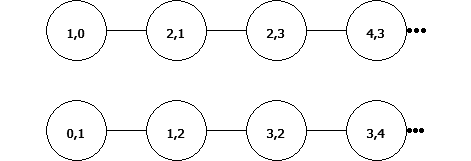
\includegraphics[height=90px]{ext/6.1.1.png}
                \caption{Граф слабоположительных решений}
                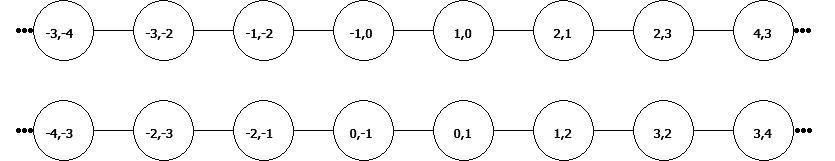
\includegraphics[height=90px]{ext/6.1.2.png}
                \caption{Граф всех решений}
            \end{Graph}

        \subsection{\large{Цикл}}
            \begin{gather*}
                f(x)=\sum_1^n x_i^2 - \sum_1^{n-1} x_i x_{i+1} - x_nx_1 = \\
                \sum_1^{n-1} \frac{1}{2}(x_i-x_{i+1})^2 + \frac{1}{2}(x_n-x_1)^2 = 1 \Rightarrow \\
                \sum_1^{n-1} (x_i-x_{i+1})^2 + (x_n-x_1)^2 = 2
            \end{gather*}
            Обозначим пару $(x_i, x_{i+1})$ (или $(x_n, x_1)$) переходом, если $|x_i-x_{i+1}| = 1$.\\
            Тогда в этом множестве ровно два перехода, а также, поскольку переходы циклические, то это значит что решение имеет форму:\\
            \begin{gather*}
                \exists\text{ } d \in \mathbb{Z} : \\
                \exists \text{ } 1 \leq i \leq j \leq n : \forall \text{ } 1 \leq k < i \text{ или } j < k \leq n : x_k = d, \forall \text{ } i \leq k \leq j : x_k = d+1.\\ \text{и}\\
                \exists \text{ } 1 \leq i \leq j \leq n : \forall \text{ } 1 \leq k < i \text{ или } j < k \leq n : x_k = d+1, \forall \text{ } i \leq k \leq j : x_k = d.
            \end{gather*}
            В таком случае граф решений будет выглядеть как множество графов аналогичных множеству решений формы бамбука связанных между собой последовательно по листьям одного с двумя вершинами другого, которые имеют единственный отличный от остальных элемент и при этом не являются листьями.
            \begin{Graph}
                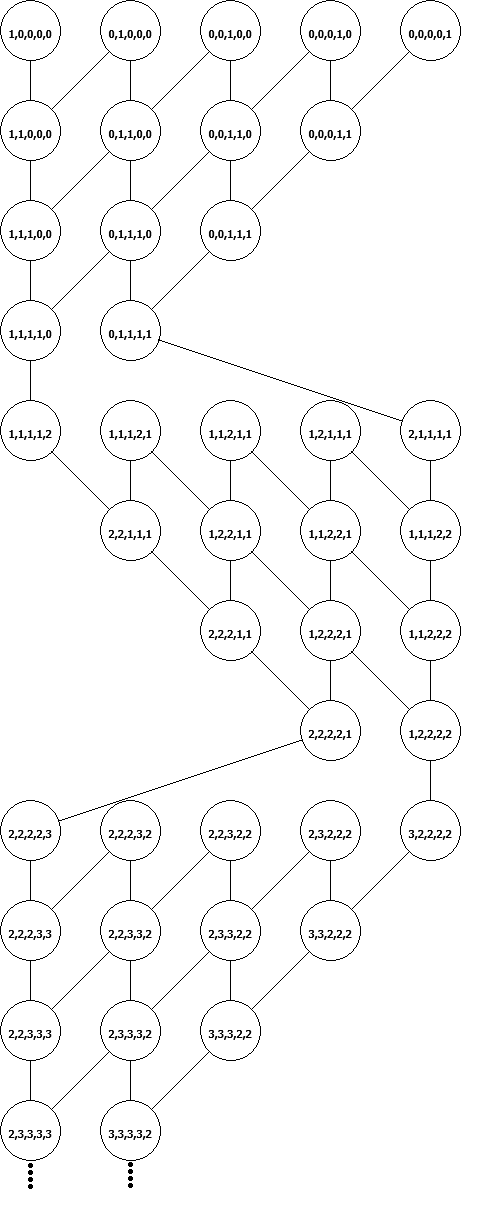
\includegraphics[height=500px]{ext/6.2.1.png}
                \caption{Граф слабоположительных решений при n = 5}
            \end{Graph}
            \pagebreak
            \begin{Graph}
                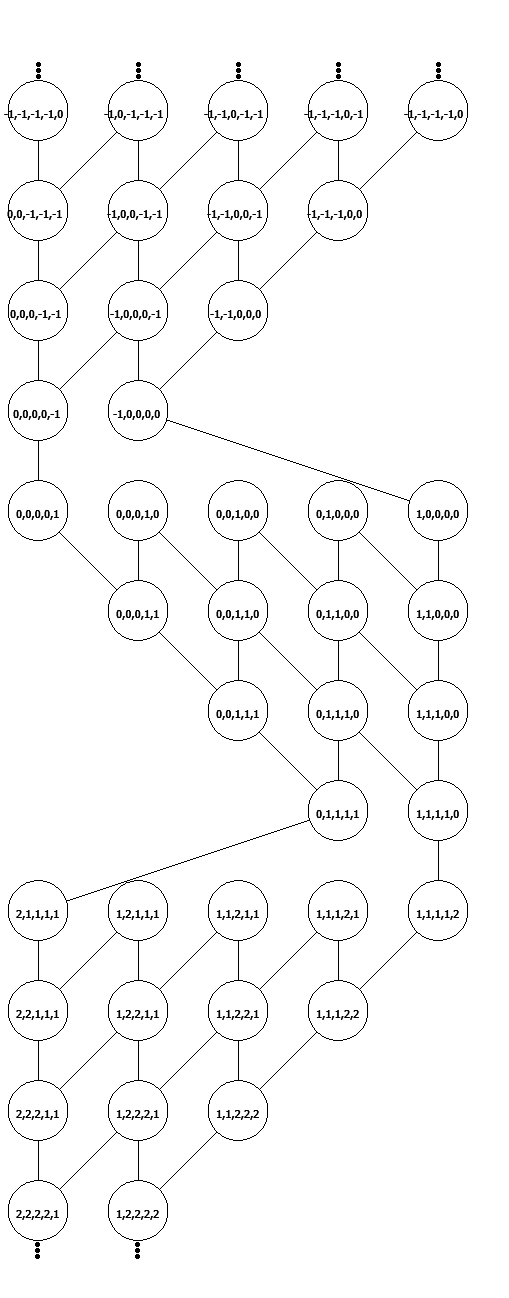
\includegraphics[height=500px]{ext/6.2.2.png}
                \caption{Граф всех решений при n = 5}
            \end{Graph}
            \pagebreak
            
        \subsection{\large{Вершина с четырьмя листьями}}
            \begin{gather*}
                f(x) = \sum_1^4x_i^2 + y^2 - y \sum_1^4 x_i = 1
            \end{gather*}
            \begin{gather*}
                f(x) = \sum_1^4 \frac{1}{4}(2x_i-y)^2 = 1
            \end{gather*}
            \begin{gather*}
                \sum_1^4(2x_i-y)^2 = 4
            \end{gather*}
            Требуется рассмотреть два случая:\\
            \begin{enumerate}
                \item $\exists \text{ } 1 \leq i \leq 4 : (2x_i-y)^2=4, \text{ } \forall \text{ } 1 \leq j \leq 4, \text{ }j \neq i : (2x_j-y)^2=0$
                \item $\forall \text{ } 1 \leq j \leq 4: (2x_j-y)^2=1$
            \end{enumerate}
            \subsubsection{}
                Если $(2x_j-y)^2=0, \text{ то } x_j = \frac{y}{2}$.
                А также, $(2x_i-y)^2=4 \Rightarrow 2x_i = y \pm 2 \Rightarrow x_i = \frac{y}{2} \pm 1$.\\
                Очевидно, решения существуют только при $y \equiv 0 \bmod 2 $.
            \subsubsection{}
                Если $(2x_i-y)^2=1, \text{ то } 2x_i=y\pm1 \Rightarrow x_i = \frac{y \pm 1}{2}$
                Очевидно, решения существуют только при $y \equiv 1 \bmod 2$.
            Тогда, граф решений можно разбить на подграфы с одинаковым y. В случае, если y чётное, то решений будет 8, если нечётное то 16. Внутри подграфов соединения не меняются от подграфа к подграфу, между подграфами y и y+1 рёбра проведены только в случаях, когда $\frac{y+1}{2} \pm 1 = \frac{y \pm 1}{2} \Rightarrow \frac{y+1}{2} - 1 = \frac{y-1}{2}$, что верно. То есть рёбра проводятся между вершинами с решениями вида $(y, \frac{y+1}{2}, \frac{y+1}{2}, \frac{y+1}{2}, \frac{y-1}{2}) \text{ и } (y+1, \frac{y+1}{2}, \frac{y+1}{2}, \frac{y+1}{2}, \frac{y+1}{2}-1)$.
            \begin{Graph}
                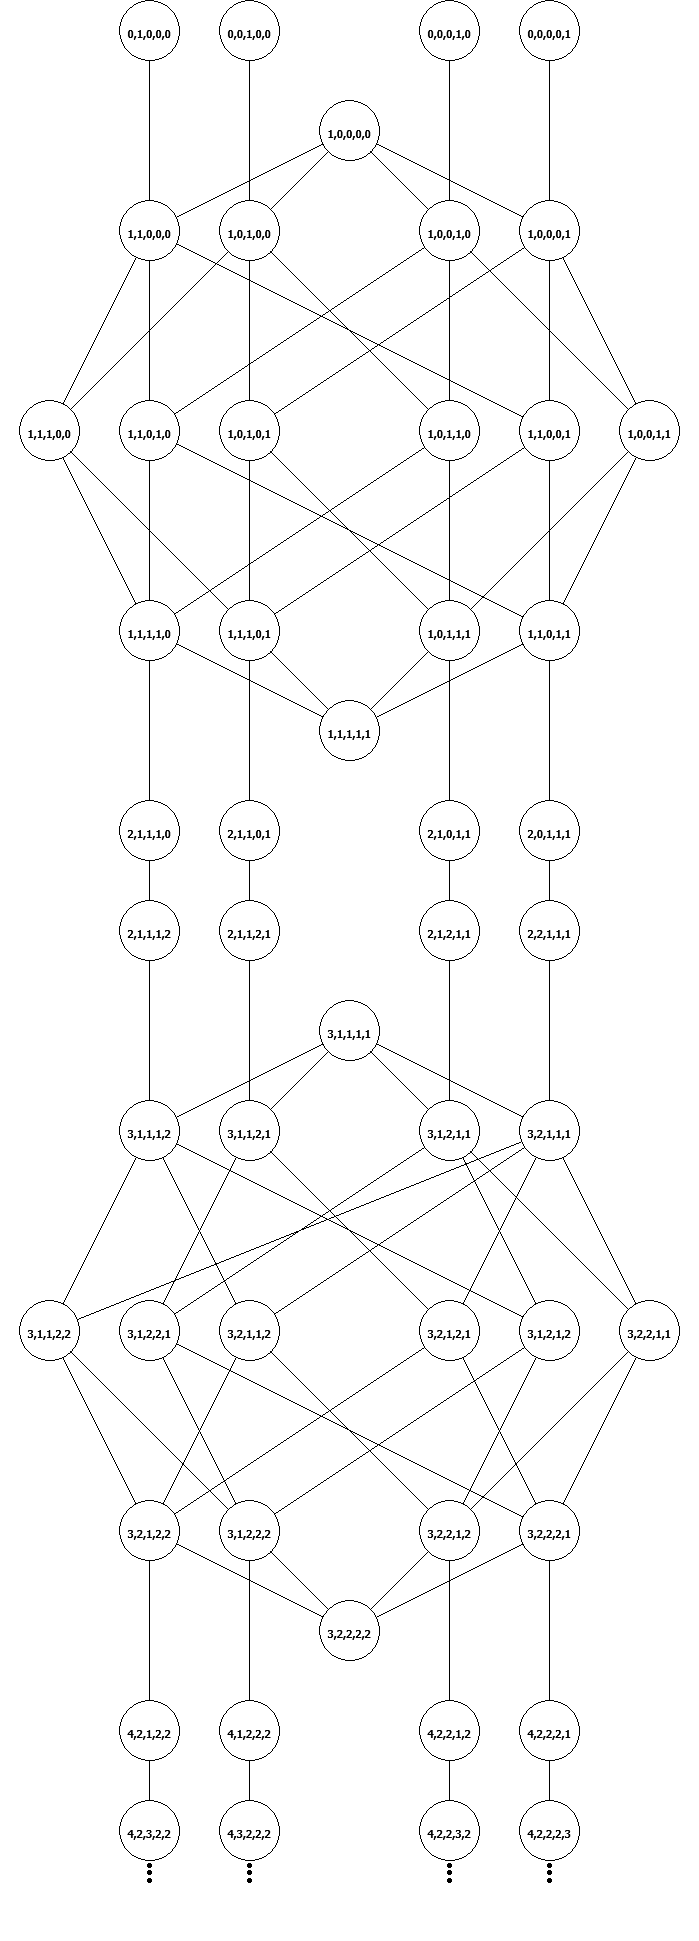
\includegraphics[height=550px]{ext/7.3.1.png}
                \caption{Граф слабоположительных решений}
            \end{Graph}
            \begin{Graph}
                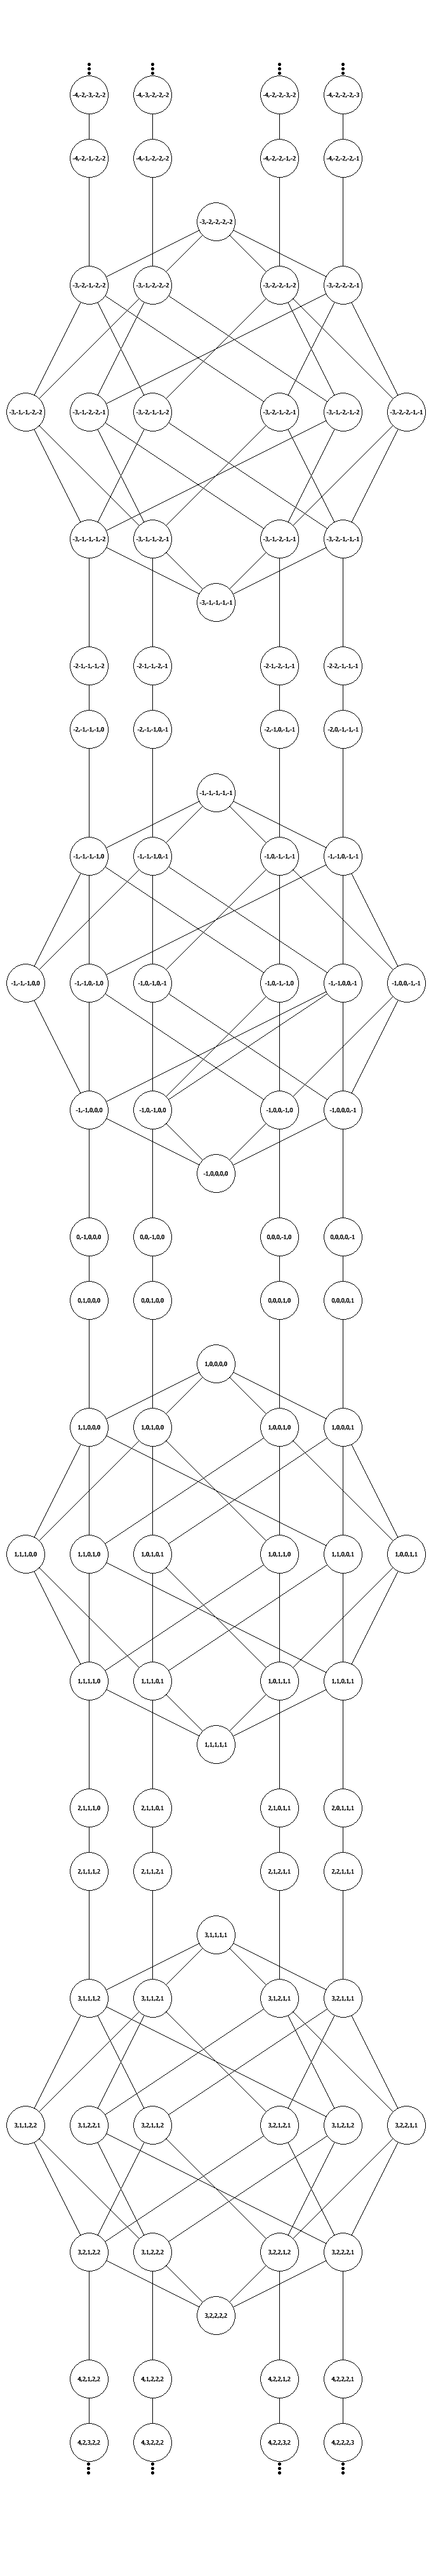
\includegraphics[height=550px]{ext/7.3.2.png}
                \caption{Граф всех решений}
            \end{Graph}
            \pagebreak
            
    \pagebreak      
    \section{\textsc{Свойства графов решений}}
        После рассмотрения всех графов решений положительных и неотрицательных форм можно сделать выводы:\\
        \begin{enumerate}
        \item Во всех таких формах граф всех решений является соединением графа слабоположительных решений и такого же графа, в котором знаки всех переменных были изменены на противоположные. Причём соединение осуществляется путём добавления ребер только между вершинами содержащими единственный ненулевой элемент (1 и -1 соответственно).
        \item Из предыдущего утверждения следует чётность количества решений и симметричность графа.
        \item Также довольно важным выводом является факт отсутсвия решений содержащий и отрицательные и положительные числа, это можно доказать без рассмотра всех графов решений, используя первый факт.
        \end{enumerate}
    \pagebreak

    \section{\textsc{Заключение}}
         В результате было выполнено:
         \begin{enumerate}
             \item Составлена классификация графов положительно определенных решений
             \item Составлена классификация графов неотрицательно определенных решений
             \item Найдены решения и графы решений положительных форм
             \item Найдены решения и графы решений неотрицательных форм
             \item Получены некоторые свойства графов решений
         \end{enumerate}
         Данный вывод может быть применен например при решении задач неявно содержащих в себе квадратичные положительно определенные формы (некоторые формы, не являющиеся положительно определенными формами, преобразуются в положительно определенные с помощью замены переменных).
    \pagebreak

    \section{\textsc{Материалы}}
    \begin{itemize} 
        \item Программа для отрисовки графов, написанная мной на
        фреймворке QT языка C++: \url{https://github.com/dmokh/Graph}
        \item Все изображения и LaTeX файлы: \url{https://github.com/dmokh/Quadratic_Forms}
    \end{itemize}
    \pagebreak

    \section{\textsc{Приложение}}
    \hypertarget{table1}{\subsection{\large{Таблица 1}}}
    \begin{longtable}{|l|l|l|l|l|l|l|c|}
    \hline
№ & $x_1$ & $x_2$ & $x_3 $& $x_4$ & $x_5$ & y & \text{Рёбра} \\
    \hline
1 & -1 & -2 & -3 & -2 & -1 & -2 & 2 \\ \hline
2 & -1 & -2 & -3 & -2 & -1 & -1 & 1, 3 \\ \hline
3 & -1 & -2 & -2 & -2 & -1 & -1 & 2, 4, 6 \\ \hline
4 & -1 & -2 & -2 & -1 & -1 & -1 & 3, 5, 7 \\ \hline
5 & -1 & -2 & -2 & -1 & 0 & -1 & 4, 8 \\ \hline
6 & -1 & -1 & -2 & -2 & -1 & -1 & 3, 7, 12 \\ \hline
7 & -1 & -1 & -2 & -1 & -1 & -1 & 4, 6, 8, 9, 13 \\ \hline
8 & -1 & -1 & -2 & -1 & 0 & -1 & 5, 7, 10, 14 \\ \hline
9 & -1 & -1 & -1 & -1 & -1 & -1 & 7, 10, 15, 22 \\ \hline
10 & -1 & -1 & -1 & -1 & 0 & -1 & 8, 9, 11, 16, 23 \\ \hline
11 & -1 & -1 & -1 & 0 & 0 & -1 & 10, 17, 24 \\ \hline
12 & 0 & -1 & -2 & -2 & -1 & -1 & 6, 13 \\ \hline
13 & 0 & -1 & -2 & -1 & -1 & -1 & 7, 12, 14, 15 \\ \hline
14 & 0 & -1 & -2 & -1 & 0 & -1 & 8, 13, 16 \\ \hline
15 & 0 & -1 & -1 & -1 & -1 & -1 & 9, 13, 16, 18, 27 \\ \hline
16 & 0 & -1 & -1 & -1 & 0 & -1 & 10, 14, 15, 17, 19, 28 \\ \hline
17 & 0 & -1 & -1 & 0 & 0 & -1 & 11, 16, 20, 29 \\ \hline
18 & 0 & 0 & -1 & -1 & -1 & -1 & 15, 19, 31 \\ \hline
19 & 0 & 0 & -1 & -1 & 0 & -1 & 16, 18, 20, 32 \\ \hline
20 & 0 & 0 & -1 & 0 & 0 & -1 & 17, 19, 21, 33 \\ \hline
21 & 0 & 0 & 0 & 0 & 0 & -1 & 20, 52 \\ \hline
22 & -1 & -1 & -1 & -1 & -1 & 0 & 9, 23, 27 \\ \hline
23 & -1 & -1 & -1 & -1 & 0 & 0 & 10, 22, 24, 28 \\ \hline
24 & -1 & -1 & -1 & 0 & 0 & 0 & 11, 23, 25, 29 \\ \hline
25 & -1 & -1 & 0 & 0 & 0 & 0 & 24, 26, 30 \\ \hline
26 & -1 & 0 & 0 & 0 & 0 & 0 & 25, 47 \\ \hline
27 & 0 & -1 & -1 & -1 & -1 & 0 & 15, 22, 28, 31 \\ \hline
28 & 0 & -1 & -1 & -1 & 0 & 0 & 16, 23, 27, 29, 32 \\ \hline
29 & 0 & -1 & -1 & 0 & 0 & 0 & 17, 24, 28, 30, 33 \\ \hline
30 & 0 & -1 & 0 & 0 & 0 & 0 & 25, 29, 43 \\ \hline
31 & 0 & 0 & -1 & -1 & -1 & 0 & 18, 27, 32, 34 \\ \hline
32 & 0 & 0 & -1 & -1 & 0 & 0 & 19, 28, 31, 33, 35 \\ \hline
33 & 0 & 0 & -1 & 0 & 0 & 0 & 20, 29, 32, 40 \\ \hline
34 & 0 & 0 & 0 & -1 & -1 & 0 & 31, 35, 36 \\ \hline
35 & 0 & 0 & 0 & -1 & 0 & 0 & 32, 34, 38 \\ \hline
36 & 0 & 0 & 0 & 0 & -1 & 0 & 34, 37 \\ \hline
37 & 0 & 0 & 0 & 0 & 1 & 0 & 36, 39 \\ \hline
38 & 0 & 0 & 0 & 1 & 0 & 0 & 35, 39, 41 \\ \hline
39 & 0 & 0 & 0 & 1 & 1 & 0 & 37, 38, 42 \\ \hline
40 & 0 & 0 & 1 & 0 & 0 & 0 & 33, 41, 44, 53 \\ \hline
41 & 0 & 0 & 1 & 1 & 0 & 0 & 38, 40, 42, 45, 54 \\ \hline
42 & 0 & 0 & 1 & 1 & 1 & 0 & 39, 41, 46, 55 \\ \hline
43 & 0 & 1 & 0 & 0 & 0 & 0 & 30, 44, 48 \\ \hline
44 & 0 & 1 & 1 & 0 & 0 & 0 & 40, 43, 45, 49, 56 \\ \hline
45 & 0 & 1 & 1 & 1 & 0 & 0 & 41, 44, 46, 50, 57 \\ \hline
46 & 0 & 1 & 1 & 1 & 1 & 0 & 42, 45, 51, 58 \\ \hline
47 & 1 & 0 & 0 & 0 & 0 & 0 & 26, 48 \\ \hline
48 & 1 & 1 & 0 & 0 & 0 & 0 & 43, 47, 49 \\ \hline
49 & 1 & 1 & 1 & 0 & 0 & 0 & 44, 48, 50, 62 \\ \hline
50 & 1 & 1 & 1 & 1 & 0 & 0 & 45, 49, 51, 63 \\ \hline
51 & 1 & 1 & 1 & 1 & 1 & 0 & 46, 50, 64 \\ \hline
52 & 0 & 0 & 0 & 0 & 0 & 1 & 21, 53 \\ \hline
53 & 0 & 0 & 1 & 0 & 0 & 1 & 40, 52, 54, 56 \\ \hline
54 & 0 & 0 & 1 & 1 & 0 & 1 & 41, 53, 55, 57 \\ \hline
55 & 0 & 0 & 1 & 1 & 1 & 1 & 42, 54, 58 \\ \hline
56 & 0 & 1 & 1 & 0 & 0 & 1 & 44, 53, 57, 62 \\ \hline
57 & 0 & 1 & 1 & 1 & 0 & 1 & 45, 54, 56, 58, 59, 63 \\ \hline
58 & 0 & 1 & 1 & 1 & 1 & 1 & 46, 55, 57, 60, 64 \\ \hline
59 & 0 & 1 & 2 & 1 & 0 & 1 & 57, 60, 65 \\ \hline
60 & 0 & 1 & 2 & 1 & 1 & 1 & 58, 59, 61, 66 \\ \hline
61 & 0 & 1 & 2 & 2 & 1 & 1 & 60, 67 \\ \hline
62 & 1 & 1 & 1 & 0 & 0 & 1 & 49, 56, 63 \\ \hline
63 & 1 & 1 & 1 & 1 & 0 & 1 & 50, 57, 62, 64, 65 \\ \hline
64 & 1 & 1 & 1 & 1 & 1 & 1 & 51, 58, 63, 66 \\ \hline
65 & 1 & 1 & 2 & 1 & 0 & 1 & 59, 63, 66, 68 \\ \hline
66 & 1 & 1 & 2 & 1 & 1 & 1 & 60, 64, 65, 67, 69 \\ \hline
67 & 1 & 1 & 2 & 2 & 1 & 1 & 61, 66, 70 \\ \hline
68 & 1 & 2 & 2 & 1 & 0 & 1 & 65, 69 \\ \hline
69 & 1 & 2 & 2 & 1 & 1 & 1 & 66, 68, 70 \\ \hline
70 & 1 & 2 & 2 & 2 & 1 & 1 & 67, 69, 71 \\ \hline
71 & 1 & 2 & 3 & 2 & 1 & 1 & 70, 72 \\ \hline
72 & 1 & 2 & 3 & 2 & 1 & 2 & 71 \\ \hline
\end{longtable}



    \newpage
    \hypertarget{table2}{\subsection{\large{Таблица 2}}}
    \begin{longtable}{|l|l|l|l|l|l|l|l|c|}
    \hline
№ & $x_1$ & $x_2$ & $x_3 $& $x_4$ & $x_5$ & $x_6$ & y & \text{Рёбра} \\
    \hline
1 & -2 & -3 & -4 & -3 & -2 & -1 & -2 & 2 \\ \hline
2 & -1 & -3 & -4 & -3 & -2 & -1 & -2 & 1, 3 \\ \hline
3 & -1 & -2 & -4 & -3 & -2 & -1 & -2 & 2, 4 \\ \hline
4 & -1 & -2 & -3 & -3 & -2 & -1 & -2 & 3, 5, 8 \\ \hline
5 & -1 & -2 & -3 & -2 & -2 & -1 & -2 & 4, 6, 9 \\ \hline
6 & -1 & -2 & -3 & -2 & -1 & -1 & -2 & 5, 7, 10 \\ \hline
7 & -1 & -2 & -3 & -2 & -1 & 0 & -2 & 6, 11 \\ \hline
8 & -1 & -2 & -3 & -3 & -2 & -1 & -1 & 4, 9 \\ \hline
9 & -1 & -2 & -3 & -2 & -2 & -1 & -1 & 5, 8, 10, 12 \\ \hline
10 & -1 & -2 & -3 & -2 & -1 & -1 & -1 & 6, 9, 11, 13 \\ \hline
11 & -1 & -2 & -3 & -2 & -1 & 0 & -1 & 7, 10, 14 \\ \hline
12 & -1 & -2 & -2 & -2 & -2 & -1 & -1 & 9, 13, 18 \\ \hline
13 & -1 & -2 & -2 & -2 & -1 & -1 & -1 & 10, 12, 14, 15, 19 \\ \hline
14 & -1 & -2 & -2 & -2 & -1 & 0 & -1 & 11, 13, 16, 20 \\ \hline
15 & -1 & -2 & -2 & -1 & -1 & -1 & -1 & 13, 16, 21 \\ \hline
16 & -1 & -2 & -2 & -1 & -1 & 0 & -1 & 14, 15, 17, 22 \\ \hline
17 & -1 & -2 & -2 & -1 & 0 & 0 & -1 & 16, 23 \\ \hline
18 & -1 & -1 & -2 & -2 & -2 & -1 & -1 & 12, 19, 28 \\ \hline
19 & -1 & -1 & -2 & -2 & -1 & -1 & -1 & 13, 18, 20, 21, 29 \\ \hline
20 & -1 & -1 & -2 & -2 & -1 & 0 & -1 & 14, 19, 22, 30 \\ \hline
21 & -1 & -1 & -2 & -1 & -1 & -1 & -1 & 15, 19, 22, 24, 31 \\ \hline
22 & -1 & -1 & -2 & -1 & -1 & 0 & -1 & 16, 20, 21, 23, 25, 32 \\ \hline
23 & -1 & -1 & -2 & -1 & 0 & 0 & -1 & 17, 22, 26, 33 \\ \hline
24 & -1 & -1 & -1 & -1 & -1 & -1 & -1 & 21, 25, 34, 43 \\ \hline
25 & -1 & -1 & -1 & -1 & -1 & 0 & -1 & 22, 24, 26, 35, 44 \\ \hline
26 & -1 & -1 & -1 & -1 & 0 & 0 & -1 & 23, 25, 27, 36, 45 \\ \hline
27 & -1 & -1 & -1 & 0 & 0 & 0 & -1 & 26, 37, 46 \\ \hline
28 & 0 & -1 & -2 & -2 & -2 & -1 & -1 & 18, 29 \\ \hline
29 & 0 & -1 & -2 & -2 & -1 & -1 & -1 & 19, 28, 30, 31 \\ \hline
30 & 0 & -1 & -2 & -2 & -1 & 0 & -1 & 20, 29, 32 \\ \hline
31 & 0 & -1 & -2 & -1 & -1 & -1 & -1 & 21, 29, 32, 34 \\ \hline
32 & 0 & -1 & -2 & -1 & -1 & 0 & -1 & 22, 30, 31, 33, 35 \\ \hline
33 & 0 & -1 & -2 & -1 & 0 & 0 & -1 & 23, 32, 36 \\ \hline
34 & 0 & -1 & -1 & -1 & -1 & -1 & -1 & 24, 31, 35, 38, 49 \\ \hline
35 & 0 & -1 & -1 & -1 & -1 & 0 & -1 & 25, 32, 34, 36, 39, 50 \\ \hline
36 & 0 & -1 & -1 & -1 & 0 & 0 & -1 & 26, 33, 35, 37, 40, 51 \\ \hline
37 & 0 & -1 & -1 & 0 & 0 & 0 & -1 & 27, 36, 41, 52 \\ \hline
38 & 0 & 0 & -1 & -1 & -1 & -1 & -1 & 34, 39, 54 \\ \hline
39 & 0 & 0 & -1 & -1 & -1 & 0 & -1 & 35, 38, 40, 55 \\ \hline
40 & 0 & 0 & -1 & -1 & 0 & 0 & -1 & 36, 39, 41, 56 \\ \hline
41 & 0 & 0 & -1 & 0 & 0 & 0 & -1 & 37, 40, 42, 57 \\ \hline
42 & 0 & 0 & 0 & 0 & 0 & 0 & -1 & 41, 85 \\ \hline
43 & -1 & -1 & -1 & -1 & -1 & -1 & 0 & 24, 44, 49 \\ \hline
44 & -1 & -1 & -1 & -1 & -1 & 0 & 0 & 25, 43, 45, 50 \\ \hline
45 & -1 & -1 & -1 & -1 & 0 & 0 & 0 & 26, 44, 46, 51 \\ \hline
46 & -1 & -1 & -1 & 0 & 0 & 0 & 0 & 27, 45, 47, 52 \\ \hline
47 & -1 & -1 & 0 & 0 & 0 & 0 & 0 & 46, 48, 53 \\ \hline
48 & -1 & 0 & 0 & 0 & 0 & 0 & 0 & 47, 79 \\ \hline
49 & 0 & -1 & -1 & -1 & -1 & -1 & 0 & 34, 43, 50, 54 \\ \hline
50 & 0 & -1 & -1 & -1 & -1 & 0 & 0 & 35, 44, 49, 51, 55 \\ \hline
51 & 0 & -1 & -1 & -1 & 0 & 0 & 0 & 36, 45, 50, 52, 56 \\ \hline
52 & 0 & -1 & -1 & 0 & 0 & 0 & 0 & 37, 46, 51, 53, 57 \\ \hline
53 & 0 & -1 & 0 & 0 & 0 & 0 & 0 & 47, 52, 74 \\ \hline
54 & 0 & 0 & -1 & -1 & -1 & -1 & 0 & 38, 49, 55, 58 \\ \hline
55 & 0 & 0 & -1 & -1 & -1 & 0 & 0 & 39, 50, 54, 56, 59 \\ \hline
56 & 0 & 0 & -1 & -1 & 0 & 0 & 0 & 40, 51, 55, 57, 60 \\ \hline
57 & 0 & 0 & -1 & 0 & 0 & 0 & 0 & 41, 52, 56, 70 \\ \hline
58 & 0 & 0 & 0 & -1 & -1 & -1 & 0 & 54, 59, 61 \\ \hline
59 & 0 & 0 & 0 & -1 & -1 & 0 & 0 & 55, 58, 60, 62 \\ \hline
60 & 0 & 0 & 0 & -1 & 0 & 0 & 0 & 56, 59, 67 \\ \hline
61 & 0 & 0 & 0 & 0 & -1 & -1 & 0 & 58, 62, 63 \\ \hline
62 & 0 & 0 & 0 & 0 & -1 & 0 & 0 & 59, 61, 65 \\ \hline
63 & 0 & 0 & 0 & 0 & 0 & -1 & 0 & 61, 64 \\ \hline
64 & 0 & 0 & 0 & 0 & 0 & 1 & 0 & 63, 66 \\ \hline
65 & 0 & 0 & 0 & 0 & 1 & 0 & 0 & 62, 66, 68 \\ \hline
66 & 0 & 0 & 0 & 0 & 1 & 1 & 0 & 64, 65, 69 \\ \hline
67 & 0 & 0 & 0 & 1 & 0 & 0 & 0 & 60, 68, 71 \\ \hline
68 & 0 & 0 & 0 & 1 & 1 & 0 & 0 & 65, 67, 69, 72 \\ \hline
69 & 0 & 0 & 0 & 1 & 1 & 1 & 0 & 66, 68, 73 \\ \hline
70 & 0 & 0 & 1 & 0 & 0 & 0 & 0 & 57, 71, 75, 86 \\ \hline
71 & 0 & 0 & 1 & 1 & 0 & 0 & 0 & 67, 70, 72, 76, 87 \\ \hline
72 & 0 & 0 & 1 & 1 & 1 & 0 & 0 & 68, 71, 73, 77, 88 \\ \hline
73 & 0 & 0 & 1 & 1 & 1 & 1 & 0 & 69, 72, 78, 89 \\ \hline
74 & 0 & 1 & 0 & 0 & 0 & 0 & 0 & 53, 75, 80 \\ \hline
75 & 0 & 1 & 1 & 0 & 0 & 0 & 0 & 70, 74, 76, 81, 90 \\ \hline
76 & 0 & 1 & 1 & 1 & 0 & 0 & 0 & 71, 75, 77, 82, 91 \\ \hline
77 & 0 & 1 & 1 & 1 & 1 & 0 & 0 & 72, 76, 78, 83, 92 \\ \hline
78 & 0 & 1 & 1 & 1 & 1 & 1 & 0 & 73, 77, 84, 93 \\ \hline
79 & 1 & 0 & 0 & 0 & 0 & 0 & 0 & 48, 80 \\ \hline
80 & 1 & 1 & 0 & 0 & 0 & 0 & 0 & 74, 79, 81 \\ \hline
81 & 1 & 1 & 1 & 0 & 0 & 0 & 0 & 75, 80, 82, 100 \\ \hline
82 & 1 & 1 & 1 & 1 & 0 & 0 & 0 & 76, 81, 83, 101 \\ \hline
83 & 1 & 1 & 1 & 1 & 1 & 0 & 0 & 77, 82, 84, 102 \\ \hline
84 & 1 & 1 & 1 & 1 & 1 & 1 & 0 & 78, 83, 103 \\ \hline
85 & 0 & 0 & 0 & 0 & 0 & 0 & 1 & 42, 86 \\ \hline
86 & 0 & 0 & 1 & 0 & 0 & 0 & 1 & 70, 85, 87, 90 \\ \hline
87 & 0 & 0 & 1 & 1 & 0 & 0 & 1 & 71, 86, 88, 91 \\ \hline
88 & 0 & 0 & 1 & 1 & 1 & 0 & 1 & 72, 87, 89, 92 \\ \hline
89 & 0 & 0 & 1 & 1 & 1 & 1 & 1 & 73, 88, 93 \\ \hline
90 & 0 & 1 & 1 & 0 & 0 & 0 & 1 & 75, 86, 91, 100 \\ \hline
91 & 0 & 1 & 1 & 1 & 0 & 0 & 1 & 76, 87, 90, 92, 94, 101 \\ \hline
92 & 0 & 1 & 1 & 1 & 1 & 0 & 1 & 77, 88, 91, 93, 95, 102 \\ \hline
93 & 0 & 1 & 1 & 1 & 1 & 1 & 1 & 78, 89, 92, 96, 103 \\ \hline
94 & 0 & 1 & 2 & 1 & 0 & 0 & 1 & 91, 95, 104 \\ \hline
95 & 0 & 1 & 2 & 1 & 1 & 0 & 1 & 92, 94, 96, 97, 105 \\ \hline
96 & 0 & 1 & 2 & 1 & 1 & 1 & 1 & 93, 95, 98, 106 \\ \hline
97 & 0 & 1 & 2 & 2 & 1 & 0 & 1 & 95, 98, 107 \\ \hline
98 & 0 & 1 & 2 & 2 & 1 & 1 & 1 & 96, 97, 99, 108 \\ \hline
99 & 0 & 1 & 2 & 2 & 2 & 1 & 1 & 98, 109 \\ \hline
100 & 1 & 1 & 1 & 0 & 0 & 0 & 1 & 81, 90, 101 \\ \hline
101 & 1 & 1 & 1 & 1 & 0 & 0 & 1 & 82, 91, 100, 102, 104 \\ \hline
102 & 1 & 1 & 1 & 1 & 1 & 0 & 1 & 83, 92, 101, 103, 105 \\ \hline
103 & 1 & 1 & 1 & 1 & 1 & 1 & 1 & 84, 93, 102, 106 \\ \hline
104 & 1 & 1 & 2 & 1 & 0 & 0 & 1 & 94, 101, 105, 110 \\ \hline
105 & 1 & 1 & 2 & 1 & 1 & 0 & 1 & 95, 102, 104, 106, 107, 111 \\ \hline
106 & 1 & 1 & 2 & 1 & 1 & 1 & 1 & 96, 103, 105, 108, 112 \\ \hline
107 & 1 & 1 & 2 & 2 & 1 & 0 & 1 & 97, 105, 108, 113 \\ \hline
108 & 1 & 1 & 2 & 2 & 1 & 1 & 1 & 98, 106, 107, 109, 114 \\ \hline
109 & 1 & 1 & 2 & 2 & 2 & 1 & 1 & 99, 108, 115 \\ \hline
110 & 1 & 2 & 2 & 1 & 0 & 0 & 1 & 104, 111 \\ \hline
111 & 1 & 2 & 2 & 1 & 1 & 0 & 1 & 105, 110, 112, 113 \\ \hline
112 & 1 & 2 & 2 & 1 & 1 & 1 & 1 & 106, 111, 114 \\ \hline
113 & 1 & 2 & 2 & 2 & 1 & 0 & 1 & 107, 111, 114, 116 \\ \hline
114 & 1 & 2 & 2 & 2 & 1 & 1 & 1 & 108, 112, 113, 115, 117 \\ \hline
115 & 1 & 2 & 2 & 2 & 2 & 1 & 1 & 109, 114, 118 \\ \hline
116 & 1 & 2 & 3 & 2 & 1 & 0 & 1 & 113, 117, 120 \\ \hline
117 & 1 & 2 & 3 & 2 & 1 & 1 & 1 & 114, 116, 118, 121 \\ \hline
118 & 1 & 2 & 3 & 2 & 2 & 1 & 1 & 115, 117, 119, 122 \\ \hline
119 & 1 & 2 & 3 & 3 & 2 & 1 & 1 & 118, 123 \\ \hline
120 & 1 & 2 & 3 & 2 & 1 & 0 & 2 & 116, 121 \\ \hline
121 & 1 & 2 & 3 & 2 & 1 & 1 & 2 & 117, 120, 122 \\ \hline
122 & 1 & 2 & 3 & 2 & 2 & 1 & 2 & 118, 121, 123 \\ \hline
123 & 1 & 2 & 3 & 3 & 2 & 1 & 2 & 119, 122, 124 \\ \hline
124 & 1 & 2 & 4 & 3 & 2 & 1 & 2 & 123, 125 \\ \hline
125 & 1 & 3 & 4 & 3 & 2 & 1 & 2 & 124, 126 \\ \hline
126 & 2 & 3 & 4 & 3 & 2 & 1 & 2 & 125 \\ \hline
\end{longtable}



    \newpage
    \hypertarget{table3}{\subsection{\large{Таблица 3}}}
    \begin{longtable}{|l|l|l|l|l|l|l|l|l|c|}
    \hline
№ & $x_1$ & $x_2$ & $x_3 $& $x_4$ & $x_5$ & $x_6$ & $x_7$ & y & \text{Рёбра} \\
    \hline
1 & -2 & -4 & -6 & -5 & -4 & -3 & -2 & -3 & 1 \\ \hline
2 & -2 & -4 & -6 & -5 & -4 & -3 & -1 & -3 & 0, 2 \\ \hline
3 & -2 & -4 & -6 & -5 & -4 & -2 & -1 & -3 & 1, 3 \\ \hline
4 & -2 & -4 & -6 & -5 & -3 & -2 & -1 & -3 & 2, 4 \\ \hline
5 & -2 & -4 & -6 & -4 & -3 & -2 & -1 & -3 & 3, 5 \\ \hline
6 & -2 & -4 & -5 & -4 & -3 & -2 & -1 & -3 & 4, 6, 8 \\ \hline
7 & -2 & -3 & -5 & -4 & -3 & -2 & -1 & -3 & 5, 7, 9 \\ \hline
8 & -1 & -3 & -5 & -4 & -3 & -2 & -1 & -3 & 6, 15 \\ \hline
9 & -2 & -4 & -5 & -4 & -3 & -2 & -1 & -2 & 5, 9 \\ \hline
10 & -2 & -3 & -5 & -4 & -3 & -2 & -1 & -2 & 6, 8, 10, 15 \\ \hline
11 & -2 & -3 & -4 & -4 & -3 & -2 & -1 & -2 & 9, 11, 16 \\ \hline
12 & -2 & -3 & -4 & -3 & -3 & -2 & -1 & -2 & 10, 12, 17 \\ \hline
13 & -2 & -3 & -4 & -3 & -2 & -2 & -1 & -2 & 11, 13, 18 \\ \hline
14 & -2 & -3 & -4 & -3 & -2 & -1 & -1 & -2 & 12, 14, 19 \\ \hline
15 & -2 & -3 & -4 & -3 & -2 & -1 & 0 & -2 & 13, 20 \\ \hline
16 & -1 & -3 & -5 & -4 & -3 & -2 & -1 & -2 & 7, 9, 16 \\ \hline
17 & -1 & -3 & -4 & -4 & -3 & -2 & -1 & -2 & 10, 15, 17, 21 \\ \hline
18 & -1 & -3 & -4 & -3 & -3 & -2 & -1 & -2 & 11, 16, 18, 22 \\ \hline
19 & -1 & -3 & -4 & -3 & -2 & -2 & -1 & -2 & 12, 17, 19, 23 \\ \hline
20 & -1 & -3 & -4 & -3 & -2 & -1 & -1 & -2 & 13, 18, 20, 24 \\ \hline
21 & -1 & -3 & -4 & -3 & -2 & -1 & 0 & -2 & 14, 19, 25 \\ \hline
22 & -1 & -2 & -4 & -4 & -3 & -2 & -1 & -2 & 16, 22 \\ \hline
23 & -1 & -2 & -4 & -3 & -3 & -2 & -1 & -2 & 17, 21, 23, 26 \\ \hline
24 & -1 & -2 & -4 & -3 & -2 & -2 & -1 & -2 & 18, 22, 24, 27 \\ \hline
25 & -1 & -2 & -4 & -3 & -2 & -1 & -1 & -2 & 19, 23, 25, 28 \\ \hline
26 & -1 & -2 & -4 & -3 & -2 & -1 & 0 & -2 & 20, 24, 29 \\ \hline
27 & -1 & -2 & -3 & -3 & -3 & -2 & -1 & -2 & 22, 27, 36 \\ \hline
28 & -1 & -2 & -3 & -3 & -2 & -2 & -1 & -2 & 23, 26, 28, 30, 37 \\ \hline
29 & -1 & -2 & -3 & -3 & -2 & -1 & -1 & -2 & 24, 27, 29, 31, 38 \\ \hline
30 & -1 & -2 & -3 & -3 & -2 & -1 & 0 & -2 & 25, 28, 32, 39 \\ \hline
31 & -1 & -2 & -3 & -2 & -2 & -2 & -1 & -2 & 27, 31, 40 \\ \hline
32 & -1 & -2 & -3 & -2 & -2 & -1 & -1 & -2 & 28, 30, 32, 33, 41 \\ \hline
33 & -1 & -2 & -3 & -2 & -2 & -1 & 0 & -2 & 29, 31, 34, 42 \\ \hline
34 & -1 & -2 & -3 & -2 & -1 & -1 & -1 & -2 & 31, 34, 43 \\ \hline
35 & -1 & -2 & -3 & -2 & -1 & -1 & 0 & -2 & 32, 33, 35, 44 \\ \hline
36 & -1 & -2 & -3 & -2 & -1 & 0 & 0 & -2 & 34, 45 \\ \hline
37 & -1 & -2 & -3 & -3 & -3 & -2 & -1 & -1 & 26, 37 \\ \hline
38 & -1 & -2 & -3 & -3 & -2 & -2 & -1 & -1 & 27, 36, 38, 40 \\ \hline
39 & -1 & -2 & -3 & -3 & -2 & -1 & -1 & -1 & 28, 37, 39, 41 \\ \hline
40 & -1 & -2 & -3 & -3 & -2 & -1 & 0 & -1 & 29, 38, 42 \\ \hline
41 & -1 & -2 & -3 & -2 & -2 & -2 & -1 & -1 & 30, 37, 41, 46 \\ \hline
42 & -1 & -2 & -3 & -2 & -2 & -1 & -1 & -1 & 31, 38, 40, 42, 43, 47 \\ \hline
43 & -1 & -2 & -3 & -2 & -2 & -1 & 0 & -1 & 32, 39, 41, 44, 48 \\ \hline
44 & -1 & -2 & -3 & -2 & -1 & -1 & -1 & -1 & 33, 41, 44, 49 \\ \hline
45 & -1 & -2 & -3 & -2 & -1 & -1 & 0 & -1 & 34, 42, 43, 45, 50 \\ \hline
46 & -1 & -2 & -3 & -2 & -1 & 0 & 0 & -1 & 35, 44, 51 \\ \hline
47 & -1 & -2 & -2 & -2 & -2 & -2 & -1 & -1 & 40, 47, 56 \\ \hline
48 & -1 & -2 & -2 & -2 & -2 & -1 & -1 & -1 & 41, 46, 48, 49, 57 \\ \hline
49 & -1 & -2 & -2 & -2 & -2 & -1 & 0 & -1 & 42, 47, 50, 58 \\ \hline
50 & -1 & -2 & -2 & -2 & -1 & -1 & -1 & -1 & 43, 47, 50, 52, 59 \\ \hline
51 & -1 & -2 & -2 & -2 & -1 & -1 & 0 & -1 & 44, 48, 49, 51, 53, 60 \\ \hline
52 & -1 & -2 & -2 & -2 & -1 & 0 & 0 & -1 & 45, 50, 54, 61 \\ \hline
53 & -1 & -2 & -2 & -1 & -1 & -1 & -1 & -1 & 49, 53, 62 \\ \hline
54 & -1 & -2 & -2 & -1 & -1 & -1 & 0 & -1 & 50, 52, 54, 63 \\ \hline
55 & -1 & -2 & -2 & -1 & -1 & 0 & 0 & -1 & 51, 53, 55, 64 \\ \hline
56 & -1 & -2 & -2 & -1 & 0 & 0 & 0 & -1 & 54, 65 \\ \hline
57 & -1 & -1 & -2 & -2 & -2 & -2 & -1 & -1 & 46, 57, 71 \\ \hline
58 & -1 & -1 & -2 & -2 & -2 & -1 & -1 & -1 & 47, 56, 58, 59, 72 \\ \hline
59 & -1 & -1 & -2 & -2 & -2 & -1 & 0 & -1 & 48, 57, 60, 73 \\ \hline
60 & -1 & -1 & -2 & -2 & -1 & -1 & -1 & -1 & 49, 57, 60, 62, 74 \\ \hline
61 & -1 & -1 & -2 & -2 & -1 & -1 & 0 & -1 & 50, 58, 59, 61, 63, 75 \\ \hline
62 & -1 & -1 & -2 & -2 & -1 & 0 & 0 & -1 & 51, 60, 64, 76 \\ \hline
63 & -1 & -1 & -2 & -1 & -1 & -1 & -1 & -1 & 52, 59, 63, 66, 77 \\ \hline
64 & -1 & -1 & -2 & -1 & -1 & -1 & 0 & -1 & 53, 60, 62, 64, 67, 78 \\ \hline
65 & -1 & -1 & -2 & -1 & -1 & 0 & 0 & -1 & 54, 61, 63, 65, 68, 79 \\ \hline
66 & -1 & -1 & -2 & -1 & 0 & 0 & 0 & -1 & 55, 64, 69, 80 \\ \hline
67 & -1 & -1 & -1 & -1 & -1 & -1 & -1 & -1 & 62, 67, 81, 92 \\ \hline
68 & -1 & -1 & -1 & -1 & -1 & -1 & 0 & -1 & 63, 66, 68, 82, 93 \\ \hline
69 & -1 & -1 & -1 & -1 & -1 & 0 & 0 & -1 & 64, 67, 69, 83, 94 \\ \hline
70 & -1 & -1 & -1 & -1 & 0 & 0 & 0 & -1 & 65, 68, 70, 84, 95 \\ \hline
71 & -1 & -1 & -1 & 0 & 0 & 0 & 0 & -1 & 69, 85, 96 \\ \hline
72 & 0 & -1 & -2 & -2 & -2 & -2 & -1 & -1 & 56, 72 \\ \hline
73 & 0 & -1 & -2 & -2 & -2 & -1 & -1 & -1 & 57, 71, 73, 74 \\ \hline
74 & 0 & -1 & -2 & -2 & -2 & -1 & 0 & -1 & 58, 72, 75 \\ \hline
75 & 0 & -1 & -2 & -2 & -1 & -1 & -1 & -1 & 59, 72, 75, 77 \\ \hline
76 & 0 & -1 & -2 & -2 & -1 & -1 & 0 & -1 & 60, 73, 74, 76, 78 \\ \hline
77 & 0 & -1 & -2 & -2 & -1 & 0 & 0 & -1 & 61, 75, 79 \\ \hline
78 & 0 & -1 & -2 & -1 & -1 & -1 & -1 & -1 & 62, 74, 78, 81 \\ \hline
79 & 0 & -1 & -2 & -1 & -1 & -1 & 0 & -1 & 63, 75, 77, 79, 82 \\ \hline
80 & 0 & -1 & -2 & -1 & -1 & 0 & 0 & -1 & 64, 76, 78, 80, 83 \\ \hline
81 & 0 & -1 & -2 & -1 & 0 & 0 & 0 & -1 & 65, 79, 84 \\ \hline
82 & 0 & -1 & -1 & -1 & -1 & -1 & -1 & -1 & 66, 77, 82, 86, 99 \\ \hline
83 & 0 & -1 & -1 & -1 & -1 & -1 & 0 & -1 & 67, 78, 81, 83, 87, 100 \\ \hline
84 & 0 & -1 & -1 & -1 & -1 & 0 & 0 & -1 & 68, 79, 82, 84, 88, 101 \\ \hline
85 & 0 & -1 & -1 & -1 & 0 & 0 & 0 & -1 & 69, 80, 83, 85, 89, 102 \\ \hline
86 & 0 & -1 & -1 & 0 & 0 & 0 & 0 & -1 & 70, 84, 90, 103 \\ \hline
87 & 0 & 0 & -1 & -1 & -1 & -1 & -1 & -1 & 81, 87, 105 \\ \hline
88 & 0 & 0 & -1 & -1 & -1 & -1 & 0 & -1 & 82, 86, 88, 106 \\ \hline
89 & 0 & 0 & -1 & -1 & -1 & 0 & 0 & -1 & 83, 87, 89, 107 \\ \hline
90 & 0 & 0 & -1 & -1 & 0 & 0 & 0 & -1 & 84, 88, 90, 108 \\ \hline
91 & 0 & 0 & -1 & 0 & 0 & 0 & 0 & -1 & 85, 89, 91, 109 \\ \hline
92 & 0 & 0 & 0 & 0 & 0 & 0 & 0 & -1 & 90, 148 \\ \hline
93 & -1 & -1 & -1 & -1 & -1 & -1 & -1 & 0 & 66, 93, 99 \\ \hline
94 & -1 & -1 & -1 & -1 & -1 & -1 & 0 & 0 & 67, 92, 94, 100 \\ \hline
95 & -1 & -1 & -1 & -1 & -1 & 0 & 0 & 0 & 68, 93, 95, 101 \\ \hline
96 & -1 & -1 & -1 & -1 & 0 & 0 & 0 & 0 & 69, 94, 96, 102 \\ \hline
97 & -1 & -1 & -1 & 0 & 0 & 0 & 0 & 0 & 70, 95, 97, 103 \\ \hline
98 & -1 & -1 & 0 & 0 & 0 & 0 & 0 & 0 & 96, 98, 104 \\ \hline
99 & -1 & 0 & 0 & 0 & 0 & 0 & 0 & 0 & 97, 141 \\ \hline
100 & 0 & -1 & -1 & -1 & -1 & -1 & -1 & 0 & 81, 92, 100, 105 \\ \hline
101 & 0 & -1 & -1 & -1 & -1 & -1 & 0 & 0 & 82, 93, 99, 101, 106 \\ \hline
102 & 0 & -1 & -1 & -1 & -1 & 0 & 0 & 0 & 83, 94, 100, 102, 107 \\ \hline
103 & 0 & -1 & -1 & -1 & 0 & 0 & 0 & 0 & 84, 95, 101, 103, 108 \\ \hline
104 & 0 & -1 & -1 & 0 & 0 & 0 & 0 & 0 & 85, 96, 102, 104, 109 \\ \hline
105 & 0 & -1 & 0 & 0 & 0 & 0 & 0 & 0 & 97, 103, 135 \\ \hline
106 & 0 & 0 & -1 & -1 & -1 & -1 & -1 & 0 & 86, 99, 106, 110 \\ \hline
107 & 0 & 0 & -1 & -1 & -1 & -1 & 0 & 0 & 87, 100, 105, 107, 111 \\ \hline
108 & 0 & 0 & -1 & -1 & -1 & 0 & 0 & 0 & 88, 101, 106, 108, 112 \\ \hline
109 & 0 & 0 & -1 & -1 & 0 & 0 & 0 & 0 & 89, 102, 107, 109, 113 \\ \hline
110 & 0 & 0 & -1 & 0 & 0 & 0 & 0 & 0 & 90, 103, 108, 130 \\ \hline
111 & 0 & 0 & 0 & -1 & -1 & -1 & -1 & 0 & 105, 111, 114 \\ \hline
112 & 0 & 0 & 0 & -1 & -1 & -1 & 0 & 0 & 106, 110, 112, 115 \\ \hline
113 & 0 & 0 & 0 & -1 & -1 & 0 & 0 & 0 & 107, 111, 113, 116 \\ \hline
114 & 0 & 0 & 0 & -1 & 0 & 0 & 0 & 0 & 108, 112, 126 \\ \hline
115 & 0 & 0 & 0 & 0 & -1 & -1 & -1 & 0 & 110, 115, 117 \\ \hline
116 & 0 & 0 & 0 & 0 & -1 & -1 & 0 & 0 & 111, 114, 116, 118 \\ \hline
117 & 0 & 0 & 0 & 0 & -1 & 0 & 0 & 0 & 112, 115, 123 \\ \hline
118 & 0 & 0 & 0 & 0 & 0 & -1 & -1 & 0 & 114, 118, 119 \\ \hline
119 & 0 & 0 & 0 & 0 & 0 & -1 & 0 & 0 & 115, 117, 121 \\ \hline
120 & 0 & 0 & 0 & 0 & 0 & 0 & -1 & 0 & 117, 120 \\ \hline
121 & 0 & 0 & 0 & 0 & 0 & 0 & 1 & 0 & 119, 122 \\ \hline
122 & 0 & 0 & 0 & 0 & 0 & 1 & 0 & 0 & 118, 122, 124 \\ \hline
123 & 0 & 0 & 0 & 0 & 0 & 1 & 1 & 0 & 120, 121, 125 \\ \hline
124 & 0 & 0 & 0 & 0 & 1 & 0 & 0 & 0 & 116, 124, 127 \\ \hline
125 & 0 & 0 & 0 & 0 & 1 & 1 & 0 & 0 & 121, 123, 125, 128 \\ \hline
126 & 0 & 0 & 0 & 0 & 1 & 1 & 1 & 0 & 122, 124, 129 \\ \hline
127 & 0 & 0 & 0 & 1 & 0 & 0 & 0 & 0 & 113, 127, 131 \\ \hline
128 & 0 & 0 & 0 & 1 & 1 & 0 & 0 & 0 & 123, 126, 128, 132 \\ \hline
129 & 0 & 0 & 0 & 1 & 1 & 1 & 0 & 0 & 124, 127, 129, 133 \\ \hline
130 & 0 & 0 & 0 & 1 & 1 & 1 & 1 & 0 & 125, 128, 134 \\ \hline
131 & 0 & 0 & 1 & 0 & 0 & 0 & 0 & 0 & 109, 131, 136, 149 \\ \hline
132 & 0 & 0 & 1 & 1 & 0 & 0 & 0 & 0 & 126, 130, 132, 137, 150 \\ \hline
133 & 0 & 0 & 1 & 1 & 1 & 0 & 0 & 0 & 127, 131, 133, 138, 151 \\ \hline
134 & 0 & 0 & 1 & 1 & 1 & 1 & 0 & 0 & 128, 132, 134, 139, 152 \\ \hline
135 & 0 & 0 & 1 & 1 & 1 & 1 & 1 & 0 & 129, 133, 140, 153 \\ \hline
136 & 0 & 1 & 0 & 0 & 0 & 0 & 0 & 0 & 104, 136, 142 \\ \hline
137 & 0 & 1 & 1 & 0 & 0 & 0 & 0 & 0 & 130, 135, 137, 143, 154 \\ \hline
138 & 0 & 1 & 1 & 1 & 0 & 0 & 0 & 0 & 131, 136, 138, 144, 155 \\ \hline
139 & 0 & 1 & 1 & 1 & 1 & 0 & 0 & 0 & 132, 137, 139, 145, 156 \\ \hline
140 & 0 & 1 & 1 & 1 & 1 & 1 & 0 & 0 & 133, 138, 140, 146, 157 \\ \hline
141 & 0 & 1 & 1 & 1 & 1 & 1 & 1 & 0 & 134, 139, 147, 158 \\ \hline
142 & 1 & 0 & 0 & 0 & 0 & 0 & 0 & 0 & 98, 142 \\ \hline
143 & 1 & 1 & 0 & 0 & 0 & 0 & 0 & 0 & 135, 141, 143 \\ \hline
144 & 1 & 1 & 1 & 0 & 0 & 0 & 0 & 0 & 136, 142, 144, 169 \\ \hline
145 & 1 & 1 & 1 & 1 & 0 & 0 & 0 & 0 & 137, 143, 145, 170 \\ \hline
146 & 1 & 1 & 1 & 1 & 1 & 0 & 0 & 0 & 138, 144, 146, 171 \\ \hline
147 & 1 & 1 & 1 & 1 & 1 & 1 & 0 & 0 & 139, 145, 147, 172 \\ \hline
148 & 1 & 1 & 1 & 1 & 1 & 1 & 1 & 0 & 140, 146, 173 \\ \hline
149 & 0 & 0 & 0 & 0 & 0 & 0 & 0 & 1 & 91, 149 \\ \hline
150 & 0 & 0 & 1 & 0 & 0 & 0 & 0 & 1 & 130, 148, 150, 154 \\ \hline
151 & 0 & 0 & 1 & 1 & 0 & 0 & 0 & 1 & 131, 149, 151, 155 \\ \hline
152 & 0 & 0 & 1 & 1 & 1 & 0 & 0 & 1 & 132, 150, 152, 156 \\ \hline
153 & 0 & 0 & 1 & 1 & 1 & 1 & 0 & 1 & 133, 151, 153, 157 \\ \hline
154 & 0 & 0 & 1 & 1 & 1 & 1 & 1 & 1 & 134, 152, 158 \\ \hline
155 & 0 & 1 & 1 & 0 & 0 & 0 & 0 & 1 & 136, 149, 155, 169 \\ \hline
156 & 0 & 1 & 1 & 1 & 0 & 0 & 0 & 1 & 137, 150, 154, 156, 159, 170 \\ \hline
157 & 0 & 1 & 1 & 1 & 1 & 0 & 0 & 1 & 138, 151, 155, 157, 160, 171 \\ \hline
158 & 0 & 1 & 1 & 1 & 1 & 1 & 0 & 1 & 139, 152, 156, 158, 161, 172 \\ \hline
159 & 0 & 1 & 1 & 1 & 1 & 1 & 1 & 1 & 140, 153, 157, 162, 173 \\ \hline
160 & 0 & 1 & 2 & 1 & 0 & 0 & 0 & 1 & 155, 160, 174 \\ \hline
161 & 0 & 1 & 2 & 1 & 1 & 0 & 0 & 1 & 156, 159, 161, 163, 175 \\ \hline
162 & 0 & 1 & 2 & 1 & 1 & 1 & 0 & 1 & 157, 160, 162, 164, 176 \\ \hline
163 & 0 & 1 & 2 & 1 & 1 & 1 & 1 & 1 & 158, 161, 165, 177 \\ \hline
164 & 0 & 1 & 2 & 2 & 1 & 0 & 0 & 1 & 160, 164, 178 \\ \hline
165 & 0 & 1 & 2 & 2 & 1 & 1 & 0 & 1 & 161, 163, 165, 166, 179 \\ \hline
166 & 0 & 1 & 2 & 2 & 1 & 1 & 1 & 1 & 162, 164, 167, 180 \\ \hline
167 & 0 & 1 & 2 & 2 & 2 & 1 & 0 & 1 & 164, 167, 181 \\ \hline
168 & 0 & 1 & 2 & 2 & 2 & 1 & 1 & 1 & 165, 166, 168, 182 \\ \hline
169 & 0 & 1 & 2 & 2 & 2 & 2 & 1 & 1 & 167, 183 \\ \hline
170 & 1 & 1 & 1 & 0 & 0 & 0 & 0 & 1 & 143, 154, 170 \\ \hline
171 & 1 & 1 & 1 & 1 & 0 & 0 & 0 & 1 & 144, 155, 169, 171, 174 \\ \hline
172 & 1 & 1 & 1 & 1 & 1 & 0 & 0 & 1 & 145, 156, 170, 172, 175 \\ \hline
173 & 1 & 1 & 1 & 1 & 1 & 1 & 0 & 1 & 146, 157, 171, 173, 176 \\ \hline
174 & 1 & 1 & 1 & 1 & 1 & 1 & 1 & 1 & 147, 158, 172, 177 \\ \hline
175 & 1 & 1 & 2 & 1 & 0 & 0 & 0 & 1 & 159, 170, 175, 184 \\ \hline
176 & 1 & 1 & 2 & 1 & 1 & 0 & 0 & 1 & 160, 171, 174, 176, 178, 185 \\ \hline
177 & 1 & 1 & 2 & 1 & 1 & 1 & 0 & 1 & 161, 172, 175, 177, 179, 186 \\ \hline
178 & 1 & 1 & 2 & 1 & 1 & 1 & 1 & 1 & 162, 173, 176, 180, 187 \\ \hline
179 & 1 & 1 & 2 & 2 & 1 & 0 & 0 & 1 & 163, 175, 179, 188 \\ \hline
180 & 1 & 1 & 2 & 2 & 1 & 1 & 0 & 1 & 164, 176, 178, 180, 181, 189 \\ \hline
181 & 1 & 1 & 2 & 2 & 1 & 1 & 1 & 1 & 165, 177, 179, 182, 190 \\ \hline
182 & 1 & 1 & 2 & 2 & 2 & 1 & 0 & 1 & 166, 179, 182, 191 \\ \hline
183 & 1 & 1 & 2 & 2 & 2 & 1 & 1 & 1 & 167, 180, 181, 183, 192 \\ \hline
184 & 1 & 1 & 2 & 2 & 2 & 2 & 1 & 1 & 168, 182, 193 \\ \hline
185 & 1 & 2 & 2 & 1 & 0 & 0 & 0 & 1 & 174, 185 \\ \hline
186 & 1 & 2 & 2 & 1 & 1 & 0 & 0 & 1 & 175, 184, 186, 188 \\ \hline
187 & 1 & 2 & 2 & 1 & 1 & 1 & 0 & 1 & 176, 185, 187, 189 \\ \hline
188 & 1 & 2 & 2 & 1 & 1 & 1 & 1 & 1 & 177, 186, 190 \\ \hline
189 & 1 & 2 & 2 & 2 & 1 & 0 & 0 & 1 & 178, 185, 189, 194 \\ \hline
190 & 1 & 2 & 2 & 2 & 1 & 1 & 0 & 1 & 179, 186, 188, 190, 191, 195 \\ \hline
191 & 1 & 2 & 2 & 2 & 1 & 1 & 1 & 1 & 180, 187, 189, 192, 196 \\ \hline
192 & 1 & 2 & 2 & 2 & 2 & 1 & 0 & 1 & 181, 189, 192, 197 \\ \hline
193 & 1 & 2 & 2 & 2 & 2 & 1 & 1 & 1 & 182, 190, 191, 193, 198 \\ \hline
194 & 1 & 2 & 2 & 2 & 2 & 2 & 1 & 1 & 183, 192, 199 \\ \hline
195 & 1 & 2 & 3 & 2 & 1 & 0 & 0 & 1 & 188, 195, 204 \\ \hline
196 & 1 & 2 & 3 & 2 & 1 & 1 & 0 & 1 & 189, 194, 196, 197, 205 \\ \hline
197 & 1 & 2 & 3 & 2 & 1 & 1 & 1 & 1 & 190, 195, 198, 206 \\ \hline
198 & 1 & 2 & 3 & 2 & 2 & 1 & 0 & 1 & 191, 195, 198, 200, 207 \\ \hline
199 & 1 & 2 & 3 & 2 & 2 & 1 & 1 & 1 & 192, 196, 197, 199, 201, 208 \\ \hline
200 & 1 & 2 & 3 & 2 & 2 & 2 & 1 & 1 & 193, 198, 202, 209 \\ \hline
201 & 1 & 2 & 3 & 3 & 2 & 1 & 0 & 1 & 197, 201, 210 \\ \hline
202 & 1 & 2 & 3 & 3 & 2 & 1 & 1 & 1 & 198, 200, 202, 211 \\ \hline
203 & 1 & 2 & 3 & 3 & 2 & 2 & 1 & 1 & 199, 201, 203, 212 \\ \hline
204 & 1 & 2 & 3 & 3 & 3 & 2 & 1 & 1 & 202, 213 \\ \hline
205 & 1 & 2 & 3 & 2 & 1 & 0 & 0 & 2 & 194, 205 \\ \hline
206 & 1 & 2 & 3 & 2 & 1 & 1 & 0 & 2 & 195, 204, 206, 207 \\ \hline
207 & 1 & 2 & 3 & 2 & 1 & 1 & 1 & 2 & 196, 205, 208 \\ \hline
208 & 1 & 2 & 3 & 2 & 2 & 1 & 0 & 2 & 197, 205, 208, 210 \\ \hline
209 & 1 & 2 & 3 & 2 & 2 & 1 & 1 & 2 & 198, 206, 207, 209, 211 \\ \hline
210 & 1 & 2 & 3 & 2 & 2 & 2 & 1 & 2 & 199, 208, 212 \\ \hline
211 & 1 & 2 & 3 & 3 & 2 & 1 & 0 & 2 & 200, 207, 211, 214 \\ \hline
212 & 1 & 2 & 3 & 3 & 2 & 1 & 1 & 2 & 201, 208, 210, 212, 215 \\ \hline
213 & 1 & 2 & 3 & 3 & 2 & 2 & 1 & 2 & 202, 209, 211, 213, 216 \\ \hline
214 & 1 & 2 & 3 & 3 & 3 & 2 & 1 & 2 & 203, 212, 217 \\ \hline
215 & 1 & 2 & 4 & 3 & 2 & 1 & 0 & 2 & 210, 215, 219 \\ \hline
216 & 1 & 2 & 4 & 3 & 2 & 1 & 1 & 2 & 211, 214, 216, 220 \\ \hline
217 & 1 & 2 & 4 & 3 & 2 & 2 & 1 & 2 & 212, 215, 217, 221 \\ \hline
218 & 1 & 2 & 4 & 3 & 3 & 2 & 1 & 2 & 213, 216, 218, 222 \\ \hline
219 & 1 & 2 & 4 & 4 & 3 & 2 & 1 & 2 & 217, 223 \\ \hline
220 & 1 & 3 & 4 & 3 & 2 & 1 & 0 & 2 & 214, 220, 225 \\ \hline
221 & 1 & 3 & 4 & 3 & 2 & 1 & 1 & 2 & 215, 219, 221, 226 \\ \hline
222 & 1 & 3 & 4 & 3 & 2 & 2 & 1 & 2 & 216, 220, 222, 227 \\ \hline
223 & 1 & 3 & 4 & 3 & 3 & 2 & 1 & 2 & 217, 221, 223, 228 \\ \hline
224 & 1 & 3 & 4 & 4 & 3 & 2 & 1 & 2 & 218, 222, 224, 229 \\ \hline
225 & 1 & 3 & 5 & 4 & 3 & 2 & 1 & 2 & 223, 230, 232 \\ \hline
226 & 2 & 3 & 4 & 3 & 2 & 1 & 0 & 2 & 219, 226 \\ \hline
227 & 2 & 3 & 4 & 3 & 2 & 1 & 1 & 2 & 220, 225, 227 \\ \hline
228 & 2 & 3 & 4 & 3 & 2 & 2 & 1 & 2 & 221, 226, 228 \\ \hline
229 & 2 & 3 & 4 & 3 & 3 & 2 & 1 & 2 & 222, 227, 229 \\ \hline
230 & 2 & 3 & 4 & 4 & 3 & 2 & 1 & 2 & 223, 228, 230 \\ \hline
231 & 2 & 3 & 5 & 4 & 3 & 2 & 1 & 2 & 224, 229, 231, 233 \\ \hline
232 & 2 & 4 & 5 & 4 & 3 & 2 & 1 & 2 & 230, 234 \\ \hline
233 & 1 & 3 & 5 & 4 & 3 & 2 & 1 & 3 & 224, 233 \\ \hline
234 & 2 & 3 & 5 & 4 & 3 & 2 & 1 & 3 & 230, 232, 234 \\ \hline
235 & 2 & 4 & 5 & 4 & 3 & 2 & 1 & 3 & 231, 233, 235 \\ \hline
236 & 2 & 4 & 6 & 4 & 3 & 2 & 1 & 3 & 234, 236 \\ \hline
237 & 2 & 4 & 6 & 5 & 3 & 2 & 1 & 3 & 235, 237 \\ \hline
238 & 2 & 4 & 6 & 5 & 4 & 2 & 1 & 3 & 236, 238 \\ \hline
239 & 2 & 4 & 6 & 5 & 4 & 3 & 1 & 3 & 237, 239 \\ \hline
240 & 2 & 4 & 6 & 5 & 4 & 3 & 2 & 3 & 238 \\ \hline

\end{longtable}
    \pagebreak
\end{document}
